\input{macro}

\renewcommand{\mytitle}{克服基于偏好的强化学习中的单调性陷阱：一种最大熵增量约束方法}
\renewcommand{\mytitleEN}{OVERCOMING THE MONOTONICITY TRAP IN PREFERENCE-BASED REINFORCEMENT LEARNING: A MAXIMUM ENTROPY INCREMENT CONSTRAINT APPROACH}

\begin{document}
\setlength{\baselineskip}{20pt}

\title{\hei\zihao{-2}\bfseries\mytitle}
\maketitle
\thispagestyle{empty}
\clearpage


\pagenumbering{Roman}

{\pagestyle{plain}
\tableofcontents
\clearpage}


\section*{摘~要}
设计有效的奖励信号是强化学习（RL）应用于复杂连续控制和具身智能的核心瓶颈。基于偏好的强化学习（PbRL）通过成对轨迹比较来学习奖励模型，但将其势函数直接应用于基于势的奖励重塑（PBRS）时，常遭遇极高的方差和早期梯度崩溃。本文揭示了这一现象的根本原因——\textbf{单调性陷阱（Monotonicity Trap）}：纯排序目标仅能保证轨迹的排序正确性，却无法约束PBRS所依赖的数值增量结构，导致神经网络极易陷入局部最优，使得势函数的增量结构发生病态扭曲。为了在不牺牲标签效率的前提下解决这一问题，我们提出两个互补的无监督正则化项：\textbf{最大熵增量约束（$\mathcal{L}_{struct}$）}通过最大化增量分布的熵，将势函数锚定在增量最均匀的结构上；\textbf{单调性铰链损失（$\mathcal{L}_{mono}$）}通过惩罚负增量，确保势函数沿轨迹方向单调递增。这两项正则化技术分别约束了增量分布的均匀性与方向性，协同作用下，能够仅依赖纯排序偏好即可恢复出利于强化学习优化的数值增量结构。在LIBERO模拟操作基准测试上的实验表明，我们的方法仅使用低成本的成对轨迹偏好标签，在帧级奖励对齐和轨迹级策略排序上均大幅超越了依赖帧级进度标签的有监督基线（VOC $r$: $0.968$ vs $0.860$，提升$12.6\%$；Kendall $\tau$: $0.696$ vs $0.504$，提升$38.1\%$）。本文表明，无需获取成本高昂的绝对进度标注，仅凭排序偏好即可恢复稳定且对RL友好的数值增量结构。

% keywords
\vspace{1em}\noindent
{\zihao{-3}\hei 关键词：}
{\zihao{-4}\song 强化学习，基于偏好的奖励模型，奖励重塑，最大熵，单调性陷阱}
\clearpage



{\centering\zihao{-2}\bfseries\sffamily \mytitleEN\par}
\vspace{1em}
\section*{ABSTRACT}
Designing effective reward signals remains the core bottleneck for applying reinforcement learning (RL) to complex continuous control and embodied intelligence. Preference-based reinforcement learning (PbRL) learns reward models through pairwise trajectory comparisons, but directly deploying its potential function into potential-based reward shaping (PBRS) often encounters extreme variance and early gradient collapse. This paper reveals the root cause of this phenomenon---the \textbf{Monotonicity Trap}: pure ranking objectives can only guarantee ordinal correctness of trajectories but cannot constrain the cardinal increment structure that PBRS relies upon, causing neural networks to easily converge to potential functions with pathologically distorted increment structures. To address this problem without sacrificing label efficiency, we propose two complementary unsupervised regularizers: a \textbf{Maximum Entropy Increment Constraint ($\mathcal{L}_{struct}$)} that maximizes the entropy of the increment distribution to enforce uniformity, and a \textbf{Monotonicity Hinge Loss ($\mathcal{L}_{mono}$)} that penalizes negative increments to ensure the potential function increases monotonically along trajectories. Together, they recover an RL-friendly cardinal increment structure from pure ordinal preferences. Experiments on the LIBERO simulated manipulation benchmark demonstrate that our method, using only cheap pairwise trajectory preference labels, surpasses fully supervised baselines that rely on frame-level progress labels on both frame-level reward alignment and trajectory-level policy ranking (VOC $r$ improved by 12.6\%, Kendall $\tau$ improved by 38.1\%). These results show that stable and RL-friendly cardinal increment structure can be recovered from ordinal preferences alone, without expensive absolute progress annotations.

% keywords
\vspace{1em}\noindent
{\zihao{-3}\hei KEYWORDS:}
{\zihao{-4}\songti \rmfamily Reinforcement Learning, Preference-based Reward Model, Reward Shaping, Maximum Entropy, Monotonicity Trap}

\clearpage



\pagenumbering{arabic}
\setcounter{page}{1}

\section{引言}

设计有效的奖励信号是将强化学习（RL）扩展到复杂连续控制与具身智能的核心瓶颈 \cite{abdelkareem2022advances}。基于偏好的强化学习（PbRL）通过成对轨迹比较习得任务进度，避免了逐帧标注的高昂代价，已成为奖励建模的重要范式 \cite{christiano2017deep}。主流方法利用 Bradley--Terry 排序损失优化状态势函数 $\Phi_\theta(s)$ \cite{brown2019extrapolating, krack2026rewarding}，并通过基于势的奖励重塑（PBRS）\cite{ng1999policy} 部署密集奖励 $F(s, a, s') = \gamma \Phi(s') - \Phi(s)$，在数学上保证最优策略不变性。

然而，将偏好学习到的势函数通过 PBRS 部署时，实践中常出现显著的优化不稳定性乃至早期梯度崩溃 \cite{liang2022rune}——即使奖励模型在轨迹排序上近乎完美，下游策略优化仍常因奖励信号的剧烈方差波动而失败。本文揭示了这一现象的根源——\textbf{单调性陷阱（Monotonicity Trap）}（\cref{fig:monotonicity_trap}）：排序目标仅保证轨迹间的排序正确性（$\Phi(\tau_w) > \Phi(\tau_l)$），却无法约束 PBRS 所依赖的逐步数值增量（$\Delta\Phi$）。在缺乏结构性约束的情况下，由于神经网络倾向于捷径学习（Shortcut Learning），模型极易收敛，但其学习到的势函数在增量分布上往往呈现出病态的扭曲：虽在轨迹级排序上完全正确，却导致早期探索区域奖励几乎消失、或在任务末期产生巨大的梯度脉冲，破坏了训练稳定性。

\begin{figure}[htb]
    \centering
    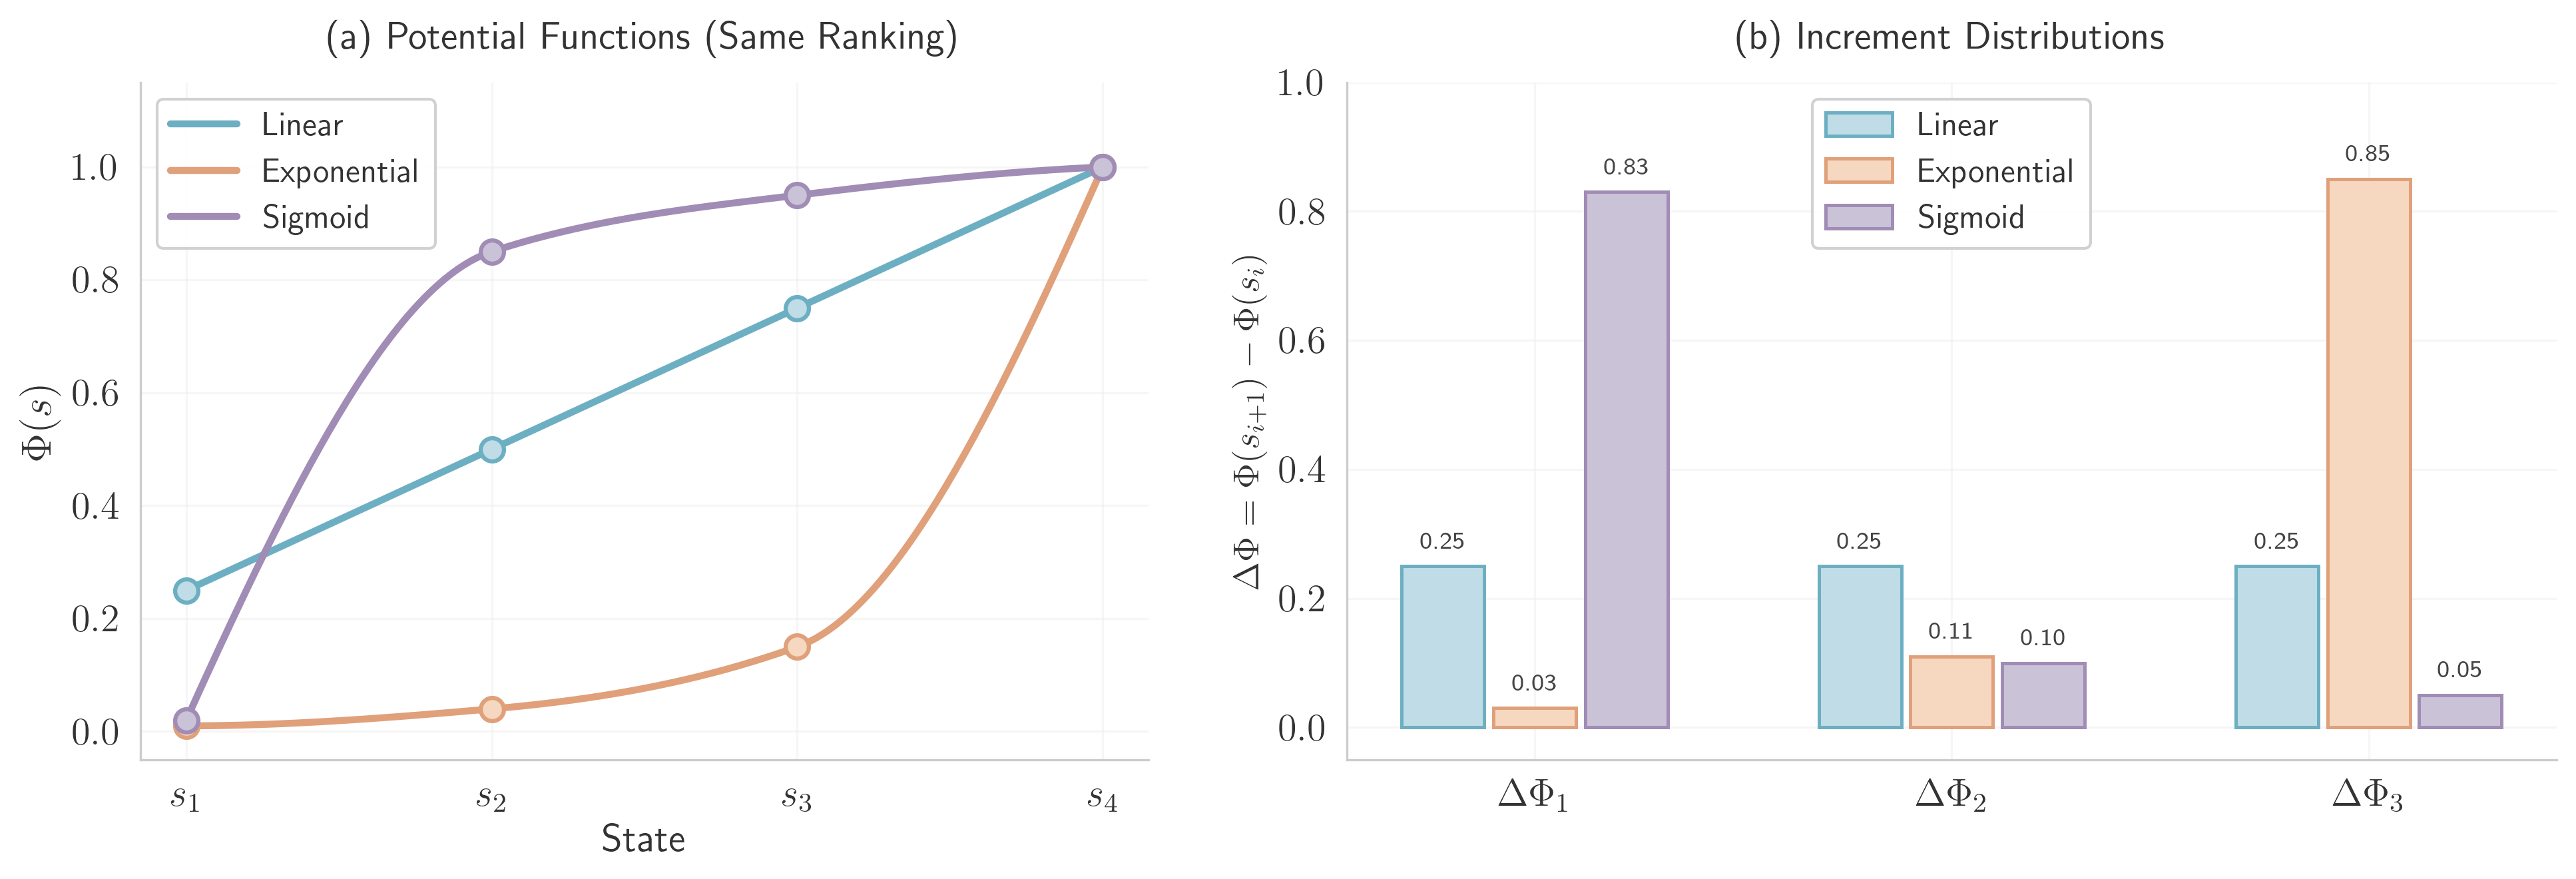
\includegraphics[width=0.95\textwidth]{figures/monotonicity-trap.png}
    \caption{\textbf{单调性陷阱及其对数值增量结构的影响。}左图展示了三种不同的势函数曲线（线性、指数、Sigmoid），它们在状态排序关系上完全等价（均满足 $\Phi(s_4) > \dots > \Phi(s_1)$），在纯排序损失（BT Loss）下具有不可识别性。右图揭示了这种排序一致性掩盖下的数值脱节：线性势产生的奖励增量 $\Delta\Phi$ 分布均匀，能提供稳定的稠密引导；指数势在任务末期产生剧烈的梯度脉冲（易导致数值爆炸）；而 Sigmoid 势则导致早期探索区域的奖励信号严重稀疏（诱发梯度消失）。这种由排序目标约束不足导致的结构性退化正是 PBRS 部署不稳定的根源。}
    \label{fig:monotonicity_trap}
\end{figure}

为弥合这一排序与数值之间的鸿沟，以 ROBOMETER \cite{robometer2026} 为代表的近期过程奖励模型引入了显式的进度标签（如时间步比率 $t/T$）来约束势函数的数值尺度。然而，这种策略面临语义对齐风险：时间步的推进并不等同于任务的真实物理进度，尤其在次优轨迹中存在大量原地徘徊或失败片段时，$t/T$ 标签会向网络注入矛盾的监督信号。

本文致力于在摒弃帧级进度标签依赖的前提下，弥合偏好学习中宏观排序目标与微观数值增量需求之间的鸿沟。核心思路在于：恢复对 RL 友好的数值增量结构，只需在排序目标上施加基于信息论的轻量级结构约束。具体地，我们引入\textbf{最大熵增量约束}（Maximum Entropy Increment Constraint, $\mathcal{L}_{struct}$），通过最大化增量分布的熵来鼓励势函数在相邻状态转换间均匀分配进度值；同时配合\textbf{单调性铰链损失}（$\mathcal{L}_{mono}$）惩罚负增量，确保势函数沿轨迹方向单调递增。两项正则化分别解决增量的均匀性和方向性问题，共同从纯排序偏好中恢复出对 RL 友好的数值增量结构。

本文的主要贡献如下：
\begin{itemize}[leftmargin=*,noitemsep]
    \item \textbf{问题诊断。}我们定义并分析了单调性陷阱：纯排序模型虽能正确排序轨迹，其帧级增量结构却发生严重退化。这揭示了 PbRL 奖励重塑不稳定的根本原因在于排序目标对数值结构的约束不足（Under-specification）。
    \item \textbf{方法设计。}我们提出两个互补的无监督正则项：$\mathcal{L}_{struct}$通过最大化增量分布的熵保证均匀性，$\mathcal{L}_{mono}$通过铰链损失保证增量方向为正。两者均无需帧级进度标注，即可从排序偏好中恢复出平滑的数值增量结构。
    \item \textbf{实验验证。}在 LIBERO 操作基准 \cite{liu2023libero} 上，本文方法仅凭成对轨迹偏好，在帧级奖励对齐（VOC $r$: $0.968$ vs $0.860$，提升$12.6\%$）和轨迹级策略排序（Kendall $\tau$: $0.696$ vs $0.504$，提升$38.1\%$）上均超越了依赖帧级进度监督的有监督基线。
\end{itemize}

\section{相关工作}

\subsection{基于偏好的奖励学习与排序约束}

从成对比较中学习奖励函数的思想最早可追溯至 Bradley-Terry 排序模型 \cite{bradley1952}。在强化学习领域，Christiano 等人 \cite{christiano2017deep} 将其扩展至深度 PbRL 框架，利用人类对轨迹片段的偏好指导策略优化。为了进一步提升标签效率，T-REX \cite{brown2019extrapolating} 提出从排序的次优演示中外推超越演示者的性能。随着大规模预训练模型的发展，RLHF 已成为大语言模型对齐的核心技术 \cite{ouyang2022training}，同时也启发了具身智能领域利用视觉语言模型（VLM）进行偏好评估的研究，如 Rewarding DINO \cite{krack2026rewarding} 和 PrefMMT \cite{zhao2025}。

然而，上述方法在优化势函数 $\Phi(s)$ 时均依赖于排序损失（Ordinal Loss）。从数学本质上看，排序目标仅确保轨迹级的累积增量 $\sum \Delta\Phi$ 满足排序关系，而无法唯一确定瞬时的数值增量（Cardinal Increments）结构。正如引言所述，这种目标固有的约束不足（Under-specification）使得神经网络极易陷入单调性陷阱：模型可能为了最小化排序损失而走“捷径”，将势函数塌陷为非线性的扭曲形态（如阶跃或指数形状）。这种退化直接导致了基于势的奖励重塑（PBRS）中奖励信号的极高方差。本文的出发点正是通过结构约束弥合排序目标与数值需求之间的鸿沟。

\subsection{过程奖励模型与进度监督}

为了缓解奖励稀疏问题，近期研究试图通过估计任务进度来构建密集的过程奖励模型（Process Reward Models, PRM）。早期方法主要依赖 VLM 的零样本评分，但由于缺乏时序连贯性，常表现出严重的时序不稳定性（Temporal Instability），即相邻帧由于视觉微变导致奖励值剧烈震荡（Value Jittering）。

后续工作如 ROBOMETER \cite{robometer2026} 试图通过显式的进度估计器来平滑信号。这类方法引入绝对进度标签（如 $t/T$）作为强监督。尽管在模拟环境下获取 $t/T$ 成本极低，但在现实机器人任务中，完成任务所需的总步数 $T$ 往往随环境干扰而动态波动，且在无标注的离线演示视频中，$T$ 的界定具有主观性。这种对帧级“特权标注”的依赖限制了模型的通用性。相比之下，我们的方法通过最大熵正则化实现无监督的结构对齐，仅需轨迹级偏好即可恢复出具有物理意义的平滑进度结构。

\subsection{基于势的奖励重塑及其正则化}
\label{sec:pbrs_regularization}

Ng 等人 \cite{ng1999policy} 提出的基于势的奖励重塑（PBRS）是PbRL中将学习到的势函数转化为重塑奖励的标准范式，其优势在于能够保持最优策略的不变性。然而，在深度 RL 的实际应用中，由于智能体策略不断演化，会引发严重的状态分布偏移（State Distribution Shift），使奖励模型在未见状态下的预测失真并产生高方差梯度 \cite{liang2022rune}。

传统的解决方案往往应用 $L_2$ 惩罚或简单的时序平滑正则化。我们指出，标准的 $L_2$ 正则化倾向于强制执行僵硬的线性插值，这往往会忽略任务中的\textbf{语义瓶颈}——即在某些关键物理动作完成瞬间（如瓶盖被拧开、夹爪精准触碰目标），奖励应当允许出现合理的非线性跃迁。我们的方法借鉴了信息论中的最大熵原理 \cite{shannon1948, jaynes1957}。不同于 $L_2$ 这种点对点的约束，最大熵增量约束作用于增量的全局概率拓扑。它允许由偏好梯度引导的、位于“语义瓶颈”处的必要奖励峰值涌现，同时确保在未定义的广阔探索区域内，奖励分布能自动平滑至最平坦的状态，从而在稳定训练与保留任务特性之间实现更优的平衡。

\section{预备知识}

\subsection{面向具身智能的马尔可夫决策过程}

我们将具身智能中的机器人操作任务建模为连续空间的马尔可夫决策过程（MDP），定义为元组 $\mathcal{M} = \langle \mathcal{S}, \mathcal{A}, \mathcal{P}, r, \gamma \rangle$ \cite{sutton2018}。在本文探讨的具身操作场景中，状态空间 $\mathcal{S}$ 通常由高维的视觉观测（如 $128 \times 128$ 的 RGB 图像像素）与低维的本体感知信息（如关节角度、末端位姿）组成；动作空间 $\mathcal{A} \in \mathbb{R}^d$ 则是连续的，代表机器人的关节速度或力矩指令。$\mathcal{P}(s'|s,a)$ 为环境动力学，$\gamma \in [0, 1)$ 为折扣因子。

为了在奖励稀疏的具身任务中加速探索，Ng 等人 \cite{ng1999policy} 提出了基于势的奖励重塑（PBRS）。给定状态势函数 $\Phi: \mathcal{S} \to \mathbb{R}$，重塑奖励定义为：
\begin{equation}
\label{eq:pbrs}
    F(s, a, s') = \gamma \Phi(s') - \Phi(s)
\end{equation}
经典理论证明，在表格型 MDP 中，该公式保证了最优策略的不变性。在深度强化学习中，尽管由于函数近似（Function Approximation）和状态分布偏移的存在，这种保证可能受到数值稳定性的挑战，但其在理论上依然提供了将“任务进度约束”转化为“稠密梯度引导”的最优路径 \cite{muller2025improving}。

\subsection{轨迹偏好学习与马尔可夫叠加假设}

在 PbRL 框架下，我们拥有一个成对偏好数据集 $\mathcal{D} = \{(\tau_1, \tau_2, y)\}$，其中 $y \in \{0, 1\}$ 表示人类或预言机对两条轨迹 $\tau = \{s_0, a_0, \dots, s_T\}$ 的优劣评判。遵循 Bradley-Terry (BT) 模型 \cite{bradley1952, christiano2017deep}，我们假设轨迹的整体偏好取决于其状态势的累积和。即轨迹 $\tau$ 的总势能定义为各帧势能的线性叠加：$\Phi(\tau) = \sum_{t=0}^T \Phi_\theta(s_t)$。

尽管这一线性叠加假设略过了任务中某些非线性的语义突破（如“物体被拿起”瞬间的特殊意义），但其赋予了奖励模型马尔可夫属性，使得下游 RL 优化在数学上是可行的。模型通过最小化交叉熵损失进行训练：
\begin{equation}
\label{eq:bt}
    \mathcal{L}_{BT} = - \mathbb{E}_{(\tau_w, \tau_l) \sim \mathcal{D}} \left[ \log \frac{\exp(\Phi_\theta(\tau_w))}{\exp(\Phi_\theta(\tau_w)) + \exp(\Phi_\theta(\tau_l))} \right]
\end{equation}

\subsection{单调性陷阱}

优化 $\mathcal{L}_{BT}$ 仅能保证势函数在“轨迹总和”尺度上的排序正确性，即满足 $\Phi_\theta(\tau_w) > \Phi_\theta(\tau_l)$。然而，这一宏观约束对微观的数值增量 $\Delta \Phi_t = \Phi_\theta(s_{t+1}) - \Phi_\theta(s_t)$ 几乎不具备结构化约束力。

我们正式定义\textbf{单调性陷阱（Monotonicity Trap）}为：在满足同一组轨迹排序约束的前提下，势函数 $\Phi_\theta(s)$ 存在无限种可能的增量分布形态。如图 \ref{fig:monotonicity_trap} 所示，模型可能收敛于一个增量分布极不均匀的势函数（如在任务末期呈指数级增长，或在初期呈阶跃式跳变）。

虽然现代 RL 算法如 PPO \cite{schulman2017} 和 SAC \cite{haarnoja2018} 具备 Advantage Normalization 和 Clipping 机制，但这些防御手段主要针对奖励的全局均值和方差进行平滑。当势函数落入单调性陷阱时，其产生的重塑奖励 $F$ 会在关键状态转换处产生极端的“奖励脉冲”（Reward Spikes）。这种局部的数值爆炸会瞬间扭曲信度分配（Credit Assignment）过程，导致梯度估计的方差超出 Clipping 的保护范围，从而引发策略的早期崩溃或陷入局部最优。下一节将提出针对这一约束不足问题的结构正则化方法。

\section{方法}

本节提出一种在离线偏好学习阶段直接约束势函数增量结构的方法。核心思路是：在不引入绝对进度标签的前提下，利用信息论结构约束防止增量退化。训练好的势函数网络在未见任务上直接泛化，无需在目标场景上重新训练或微调。

\subsection{最大熵增量约束}

如第\ref{sec:pbrs_regularization}节所述，$L_2$时间平滑惩罚是约束增量分布的常见手段，但其逐点回归的刚性本质倾向于将势函数压缩为线性插值，无法区分病态扭曲与任务中固有的语义瓶颈——即关键物理转折处（如夹爪成功抓住物体）奖励信号应当出现的合理非线性跃迁。

为了在防止病态退化的同时保留数据驱动的灵活进度分配，我们基于最大熵原理\cite{shannon1948,jaynes1957}，转向对增量序列的全局概率结构施加约束：在缺乏任务进度先验信息的情况下，基于最大熵原理的最优约束策略，应当将进度尽可能均匀地分配于相邻的状态转换之中。

对于长度为$T$的轨迹$\tau \in \mathcal{D}$，首先计算势函数的逐步增量：
\begin{equation}
\label{eq:delta_phi}
    \Delta\Phi_t = \Phi_\theta(s_{t+1}) - \Phi_\theta(s_t)
\end{equation}

由于增量$\Delta\Phi_t$的取值范围无界，不能直接计算其熵。我们通过温度缩放的Softmax将增量序列映射为概率分布：
\begin{equation}
\label{eq:softmax}
    p_t = \frac{\exp(\Delta\Phi_t / \alpha)}{\sum_{i=0}^{T-1} \exp(\Delta\Phi_i / \alpha)}
\end{equation}
其中$\alpha > 0$为温度超参数。较小的$\alpha$能放大增量间的微小差异，避免网络输出量级相近时的梯度饱和（具体分析见第\ref{sec:training_dynamics}节）。所有实验取$\alpha = 0.1$。

在此基础上，定义最大熵增量约束$\mathcal{L}_{struct}$为增量概率分布的负香农熵：
\begin{equation}
\label{eq:lstruct}
    \mathcal{L}_{struct} = \mathbb{E}_{\tau \sim \mathcal{D}} \left[ \sum_{t=0}^{T-1} p_t \log p_t \right]
\end{equation}

最小化$\mathcal{L}_{struct}$等价于最大化增量分布的熵，即鼓励模型在相邻状态转换间分配尽可能均匀的进度值。与$L_2$逐点约束不同，$\mathcal{L}_{struct}$作用于增量的全局概率结构：它允许语义瓶颈处由偏好梯度驱动的必要奖励峰值自然涌现，同时确保在广阔探索区域中增量分布自动趋向最均匀的形态。

\subsection{单调性铰链损失}

$\mathcal{L}_{struct}$通过最大化增量分布的熵来鼓励进度均匀分配，但Softmax熵具有方向不变性——它无法区分"所有增量均匀为正"与"所有增量均匀为负"。实验表明，在缺乏方向约束时，模型倾向于学习均匀递减的势函数（详见第\ref{sec:direction}节），尽管其满足熵最大化目标，却导致PBRS奖励信号方向反转。为此，我们引入单调性铰链损失：
\begin{equation}
\label{eq:lmono}
    \mathcal{L}_{mono} = \mathbb{E}_{\tau \sim \mathcal{D}} \left[ \frac{1}{T-1}\sum_{t=0}^{T-2} \max(0, -\Delta\Phi_t) \right]
\end{equation}

$\mathcal{L}_{mono}$作为铰链损失是一种柔性惩罚而非硬约束：它仅对负增量施加线性代价，不约束正增量的大小。该损失对所有训练轨迹统一计算，鼓励势函数整体趋向非递减。对于成功轨迹，这一约束直接反映物理进度的单调递增特性；对于失败轨迹，它则作为一种温和的结构约束，避免势函数学习到全局递减的退化模式。$\mathcal{L}_{struct}$与$\mathcal{L}_{mono}$在功能上互补——前者约束增量分布的均匀性，后者则保证增量的正向单调性。

\subsection{联合优化目标}
\label{sec:joint_objective}

势函数网络$\Phi_\theta$通过最小化以下复合损失进行端到端训练：
\begin{equation}
\label{eq:total_loss}
    \mathcal{L}_{total} = \mathcal{L}_{BT} + \lambda_{struct} \mathcal{L}_{struct} + \lambda_{mono} \mathcal{L}_{mono}
\end{equation}
其中$\lambda_{struct}$和$\lambda_{mono}$分别控制均匀性正则化和方向约束的强度。三项损失在功能上天然互补：$\mathcal{L}_{BT}$确保轨迹间的排序正确，$\mathcal{L}_{struct}$规范增量的均匀分布，$\mathcal{L}_{mono}$保证增量方向为正。所有实验取$\lambda_{struct} = 0.1$、$\lambda_{mono} = 0.1$。训练动态实验（\cref{tab:dynamics}）证实三项损失在训练过程中同步收敛、互不干扰。超参数的敏感性讨论见第\ref{sec:training_dynamics}节。

\subsection{下游RL部署与泛化}

离线训练收敛后，势函数网络$\Phi_\theta$的参数冻结，直接在未见的目标任务上进行泛化评估。在PBRS框架下，智能体在每步接收密集重塑奖励：
\begin{equation}
\label{eq:deploy}
    F(s_t, a_t, s_{t+1}) = \gamma \Phi_\theta(s_{t+1}) - \Phi_\theta(s_t)
\end{equation}
PBRS的策略不变性保证了重塑奖励不会引入奖励作弊。本文实验在LIBERO-90（未见任务集）上评估奖励模型的帧级对齐和轨迹级排序质量，验证结构正则化带来的增量改善能否跨任务泛化。在线RL部署验证留作未来工作（详见第\ref{sec:conclusion}节）。



\clearpage

\section{实验}

实验围绕两个核心问题展开：\textbf{（Q1）}单调性陷阱在实际训练中是否真实存在且可测量？\textbf{（Q2）}$\mathcal{L}_{struct}$能否在不借助帧级标签的前提下恢复对RL友好的数值增量结构？

\subsection{实验设置}

\textbf{基准测试。}所有实验在LIBERO模拟操作基准\cite{liu2023libero}上进行。遵循ROBOMETER的消融协议\cite{robometer2026}，训练集由LIBERO-\{10, Object, Goal, Spatial\}中的1,709条成功演示和1,929条生成的失败轨迹组成；评估在LIBERO-90上进行，该子集包含8,262对跨越未见任务的成功与失败轨迹。

\begin{figure}[htb]
    \centering
    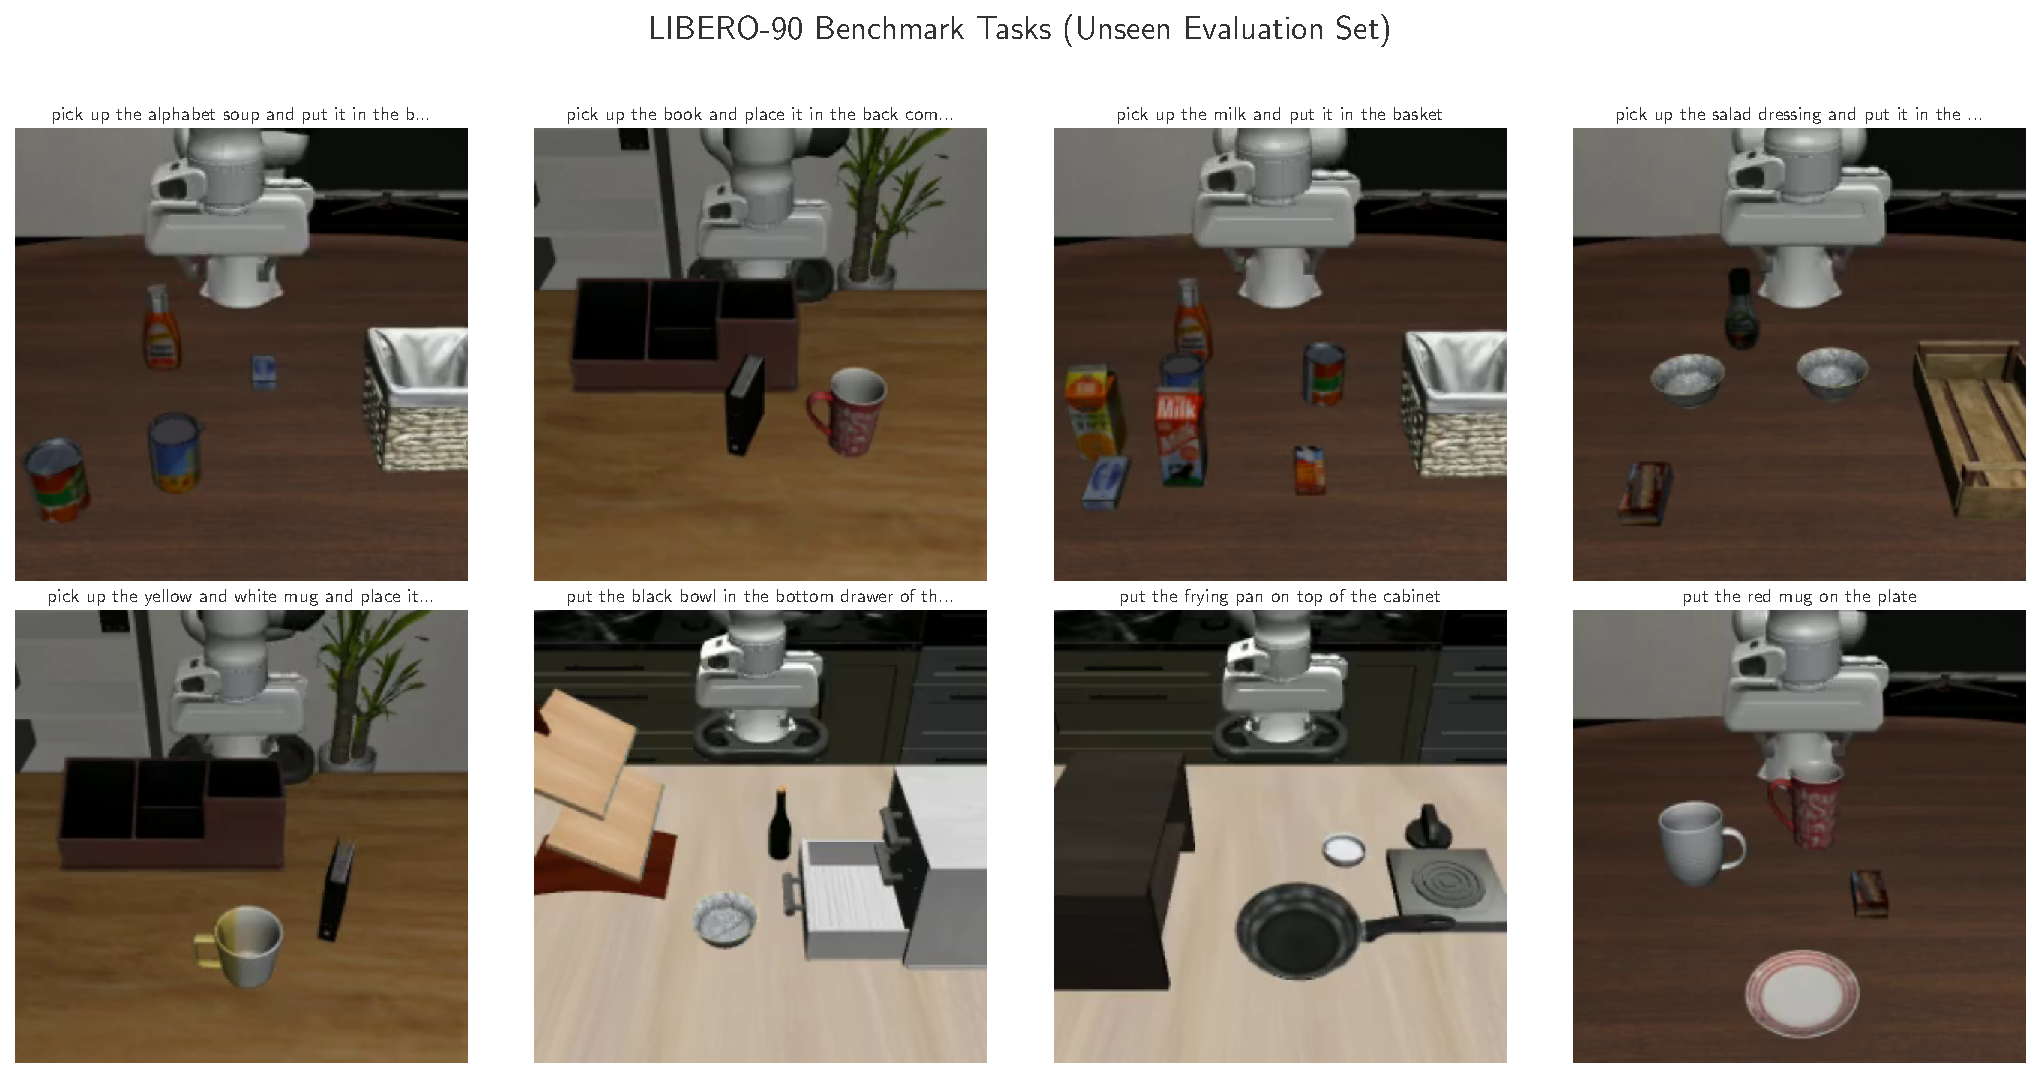
\includegraphics[width=0.95\textwidth]{figures/fig1_libero_overview_v1.pdf}
    \caption{LIBERO-90基准测试中的代表性机器人操作任务。每个子图展示了一个不同的操作任务场景，涵盖抓取、放置、堆叠等多种技能。模型在LIBERO-\{10, Object, Goal, Spatial\}上训练，在此未见的LIBERO-90任务集上进行零样本评估。}
    \label{fig:libero_overview}
\end{figure}

\textbf{基础模型与训练。}所有奖励模型变体均基于SmolVLM-500M-Instruct \cite{marafioti2025smolvlm}进行全参数微调（不使用LoRA）。SmolVLM是HuggingFace发布的紧凑型视觉语言模型，采用SigLIP视觉编码器与小型语言模型的组合架构，在多模态理解任务上展现了优良的参数效率。训练时每条轨迹子采样8帧，以多图像模式输入，批量大小为16，学习率$4 \times 10^{-5}$，余弦调度（10\%预热），共训练1,000步（单张RTX 4080 Super GPU上约55分钟）。遵循VLM微调的通行做法\cite{robometer2026,krack2026rewarding}，视觉编码器冻结，仅训练语言模型和任务预测头。图像分辨率设置为384px。

\textbf{评价指标。}采用奖励模型文献中的四个标准指标\cite{ma2024generative,robometer2026}：
\begin{itemize}[leftmargin=*,noitemsep]
    \item \textbf{VOC $r$（奖励对齐）}：值序相关系数（Value Order Correlation）\cite{ma2024generative}，定义为成功轨迹上逐帧预测奖励与时间步索引的皮尔逊相关系数（$r \in [-1, 1]$）。该指标衡量势函数是否沿成功执行呈单调递增趋势。
    \item \textbf{Kendall $\tau$（策略排序）}：Kendall秩相关系数，衡量模型对轨迹级奖励的排序与真实质量排序的一致性。
    \item \textbf{排序准确率（Ranking Accuracy）}：在成对比较中，模型将更高奖励分配给更优轨迹的正确率。
    \item \textbf{成败差异（Suc-Fail Diff）}：成功与失败轨迹的平均预测奖励之差。差值越大，说明模型对轨迹质量的区分越清晰。
\end{itemize}

\textbf{比较方法。}我们构建了四个奖励模型变体进行受控消融（\cref{tab:methods}）。

\begin{table}[ht]
    \centering
    \caption{四种比较方法的配置。前三种仅使用成对偏好标签，有监督基线额外使用帧级进度标签，构成监督水平上的上界参照。}
    \label{tab:methods}
    \resizebox{\textwidth}{!}{%
    \begin{tabular}{llll}
    \toprule
    \textbf{方法} & \textbf{架构} & \textbf{训练目标} & \textbf{所需标签} \\
    \midrule
    纯BT基线 & VLM+进度头 & $\mathcal{L}_{BT}(\sum\Phi)$ & 成对偏好 \\
    BT+L2平滑 & VLM+进度头 & $\mathcal{L}_{BT}+\lambda\cdot\mathcal{L}_{L2}$ & 成对偏好 \\
    \textbf{本文方法（BT+MaxEnt）} & VLM+进度头 & $\mathcal{L}_{BT}+\lambda\cdot\mathcal{L}_{struct}+\mathcal{L}_{mono}$ & 成对偏好 \\
    \midrule
    有监督基线（ROBOMETER） & VLM+偏好头+进度头 & $\mathcal{L}_{BT}^{head}+\mathcal{L}_{progress}$ & 成对偏好+帧级进度 \\
    \bottomrule
    \end{tabular}}
\end{table}

前三种方法共享完全相同的模型架构：一个每帧势函数$\Phi_\theta$（无Sigmoid激活的进度头），帧上求和得到轨迹级排序分数$\Phi(\tau) = \sum_{t} \Phi_\theta(s_t)$。三者的唯一区别在于损失函数：纯BT基线不加任何正则化；BT+L2平滑以$\mathcal{L}_{L2} = \sum_t (\Delta\Phi_t - \overline{\Delta\Phi})^2$鼓励增量均匀；本文方法使用$\mathcal{L}_{struct}$配合$\mathcal{L}_{mono}$。有监督基线采用ROBOMETER原始架构，包含独立的偏好头和在帧级时间步比率（$t/T$）上训练的监督进度头。该方法使用了严格多于前三者的标注信息（帧级进度标签），因此在监督水平上构成上界参照——但这并不意味着它在所有指标上必然最优。L2正则化权重设为$\lambda = 0.1$；本文方法的超参数设置见第\ref{sec:joint_objective}节。熵Softmax温度$\alpha = 0.1$。

\subsection{核心结果}

\cref{tab:main_results}给出了LIBERO-90上的评估结果。VOC $r$反映帧级奖励对齐质量（越高表示进度曲线越接近理想的线性增长），Kendall $\tau$与排序准确率衡量轨迹级排序质量，成败差异衡量成功与失败轨迹的分离程度。各列加粗值为最优。

\begin{table}[ht]
    \centering
    \caption{LIBERO-90上的奖励模型评估结果。加粗表示各列最优值。}
    \label{tab:main_results}
    \makebox[\textwidth][c]{%
    \begin{tabular}{lcccc}
    \toprule
    \textbf{方法} & \textbf{VOC $r$ $\uparrow$} & \textbf{Kendall $\tau$ $\uparrow$} & \textbf{排序准确率 $\uparrow$} & \textbf{成败差异 $\uparrow$} \\
    \midrule
    纯BT基线 & 0.147 & 0.680 & 0.840 & 14.939 \\
    BT+L2平滑 & 0.616 & \textbf{0.696} & \textbf{0.848} & \textbf{15.087} \\
    \textbf{本文方法（BT+MaxEnt）} & \textbf{0.968} & \textbf{0.696} & \textbf{0.848} & 10.800 \\
    \midrule
    有监督基线（ROBOMETER） & 0.860 & 0.504 & 0.752 & 2.175 \\
    \bottomrule
    \end{tabular}}
\end{table}

\begin{figure}[htb]
    \centering
    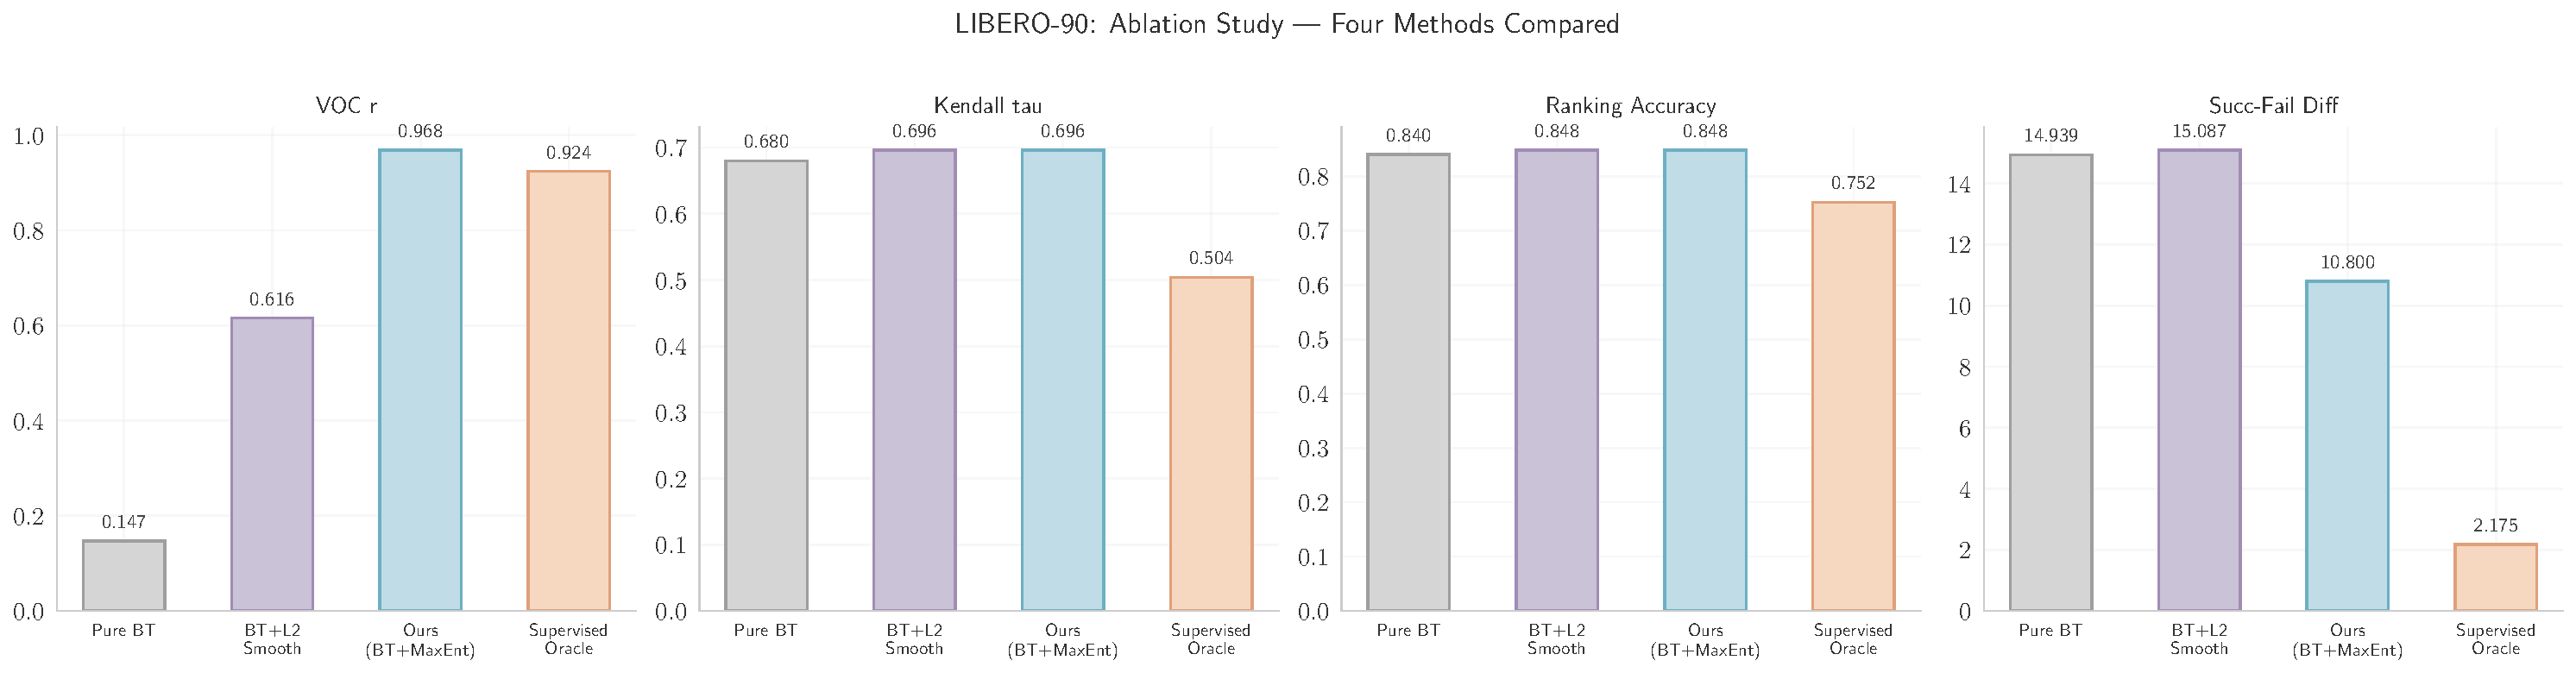
\includegraphics[width=0.95\textwidth]{figures/fig4_main_results_bar_v3.pdf}
    \caption{LIBERO-90上四种方法的定量对比。纯BT基线的VOC $r$极低（0.147），验证了单调性陷阱的存在；L2平滑有所改善但仍不充分（0.616）；本文方法以0.968大幅领先，甚至超越了使用帧级进度标签的有监督基线（0.860）。}
    \label{fig:main_results_bar}
\end{figure}

\begin{enumerate}[leftmargin=*]
    \item \textbf{本文方法在帧级对齐上大幅领先。}VOC $r = 0.968$远高于纯BT基线（$0.147$）、L2平滑（$0.616$）和有监督基线（$0.860$）。仅使用成对偏好标签，$\mathcal{L}_{struct}$配合$\mathcal{L}_{mono}$恢复的数值增量结构甚至优于帧级监督。

    \item \textbf{单调性陷阱得到实验验证。}纯BT基线的轨迹级排序尚可（Kendall $\tau = 0.680$，排序准确率$= 0.840$），但VOC $r$仅$0.147$——势函数能正确排序整条轨迹，却产生不了合理的逐帧进度结构。这正是\cref{fig:monotonicity_trap}所描述的现象：排序正确性与增量结构质量完全脱耦。

    \item \textbf{L2平滑不足以解决问题。}L2平滑将VOC $r$从$0.147$提升至$0.616$，说明时间平滑确实有助于缓解增量方差，但它只约束增量幅度应均匀，不解决方向问题——增量完全可以均匀地为负（详见第\ref{sec:direction}节的分析）。

    \item \textbf{排序能力与增量结构质量独立变化。}三种BT方法的轨迹级排序几乎相同（Kendall $\tau$：$0.680$--$0.696$），但VOC $r$从$0.147$阶梯式上升到$0.968$。这直接验证了本文的核心论点：正则化策略决定增量结构的质量，与排序能力本身无关。值得注意的是，纯BT基线和L2平滑的成败差异略高于本文方法（$14.9$/$15.1$ vs $10.8$），这是$\mathcal{L}_{mono}$使增量更均匀分布的预期代价——以少量成败分离度换取了大幅提升的帧级对齐质量。
\end{enumerate}

\begin{figure}[htb]
    \centering
    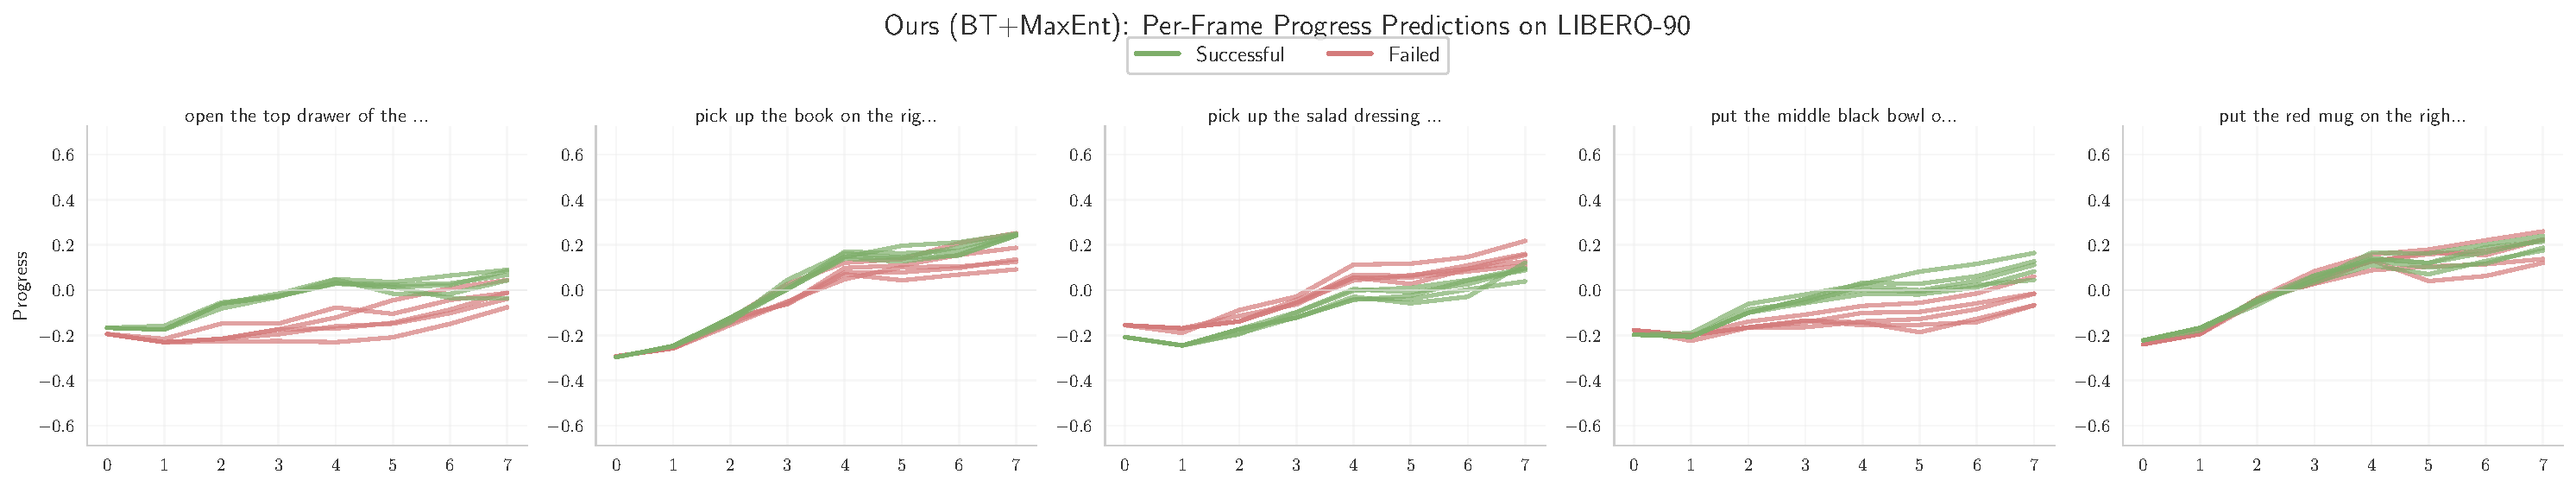
\includegraphics[width=0.95\textwidth]{figures/fig2_progress_curves_v3.pdf}
    \caption{本文方法（BT+MaxEnt）在LIBERO-90上的逐帧进度预测。绿色曲线为成功轨迹，红色为失败轨迹。成功轨迹的进度呈平滑的单调递增趋势，失败轨迹的进度则明显较低或停滞不前，表明模型有效地区分了不同质量的执行过程。}
    \label{fig:progress_curves}
\end{figure}

\begin{figure}[htb]
    \centering
    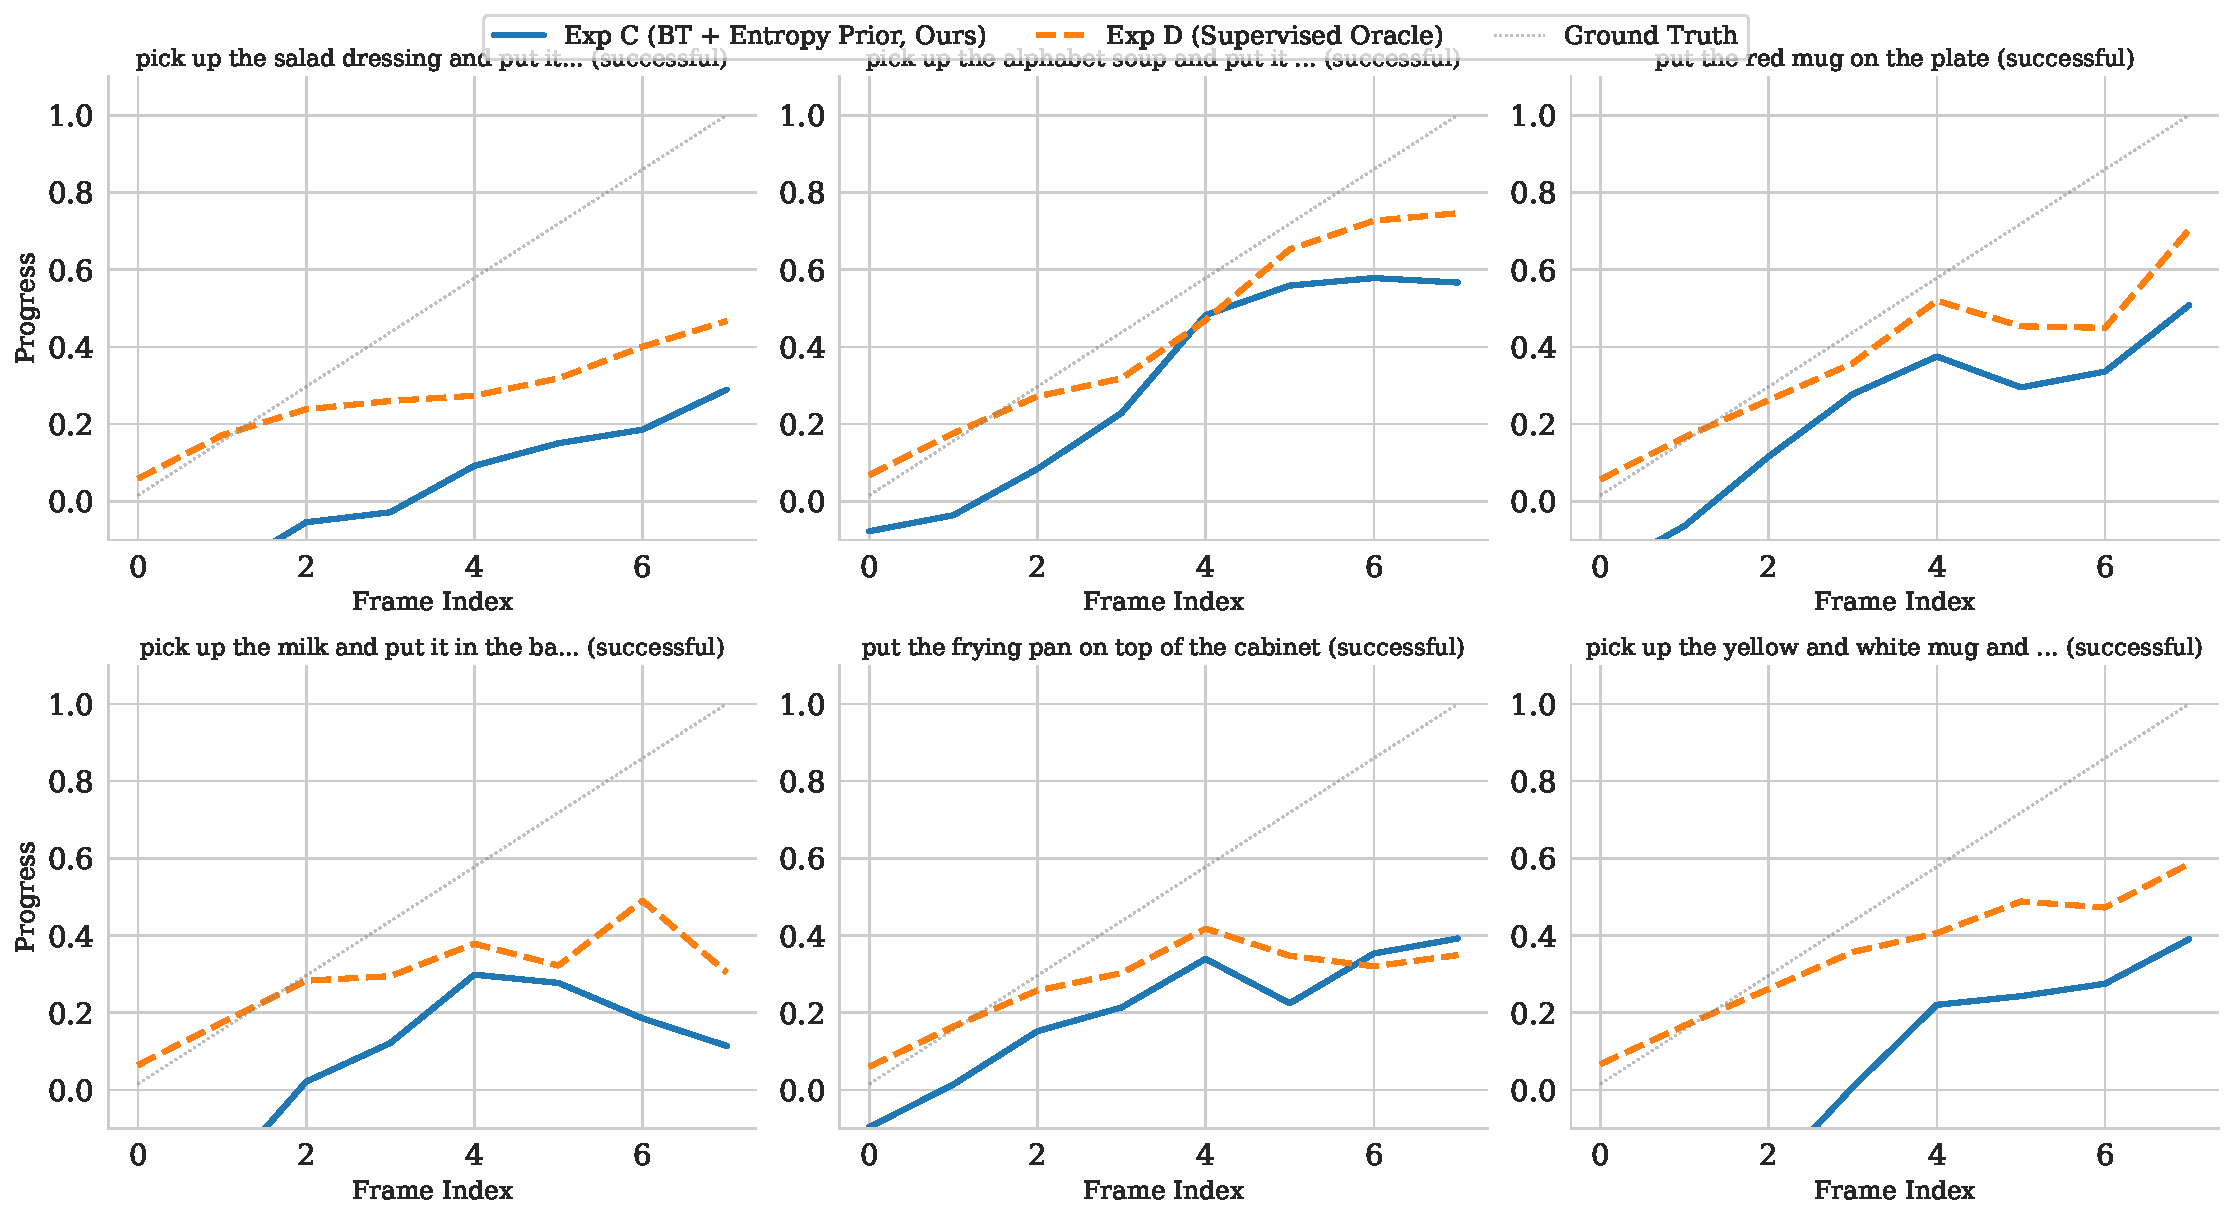
\includegraphics[width=0.95\textwidth]{figures/fig3_exp_c_vs_d_v2.pdf}
    \caption{同一批轨迹上本文方法（蓝色实线）与有监督基线（橙色虚线）的进度预测对比。灰色点线为真实时间步索引（线性进度基准）。本文方法的进度曲线与对角线高度吻合（VOC $r = 0.968$），对齐程度优于使用帧级监督信号的有监督基线（VOC $r = 0.860$）。}
    \label{fig:exp_c_vs_d}
\end{figure}

\begin{figure}[htb]
    \centering
    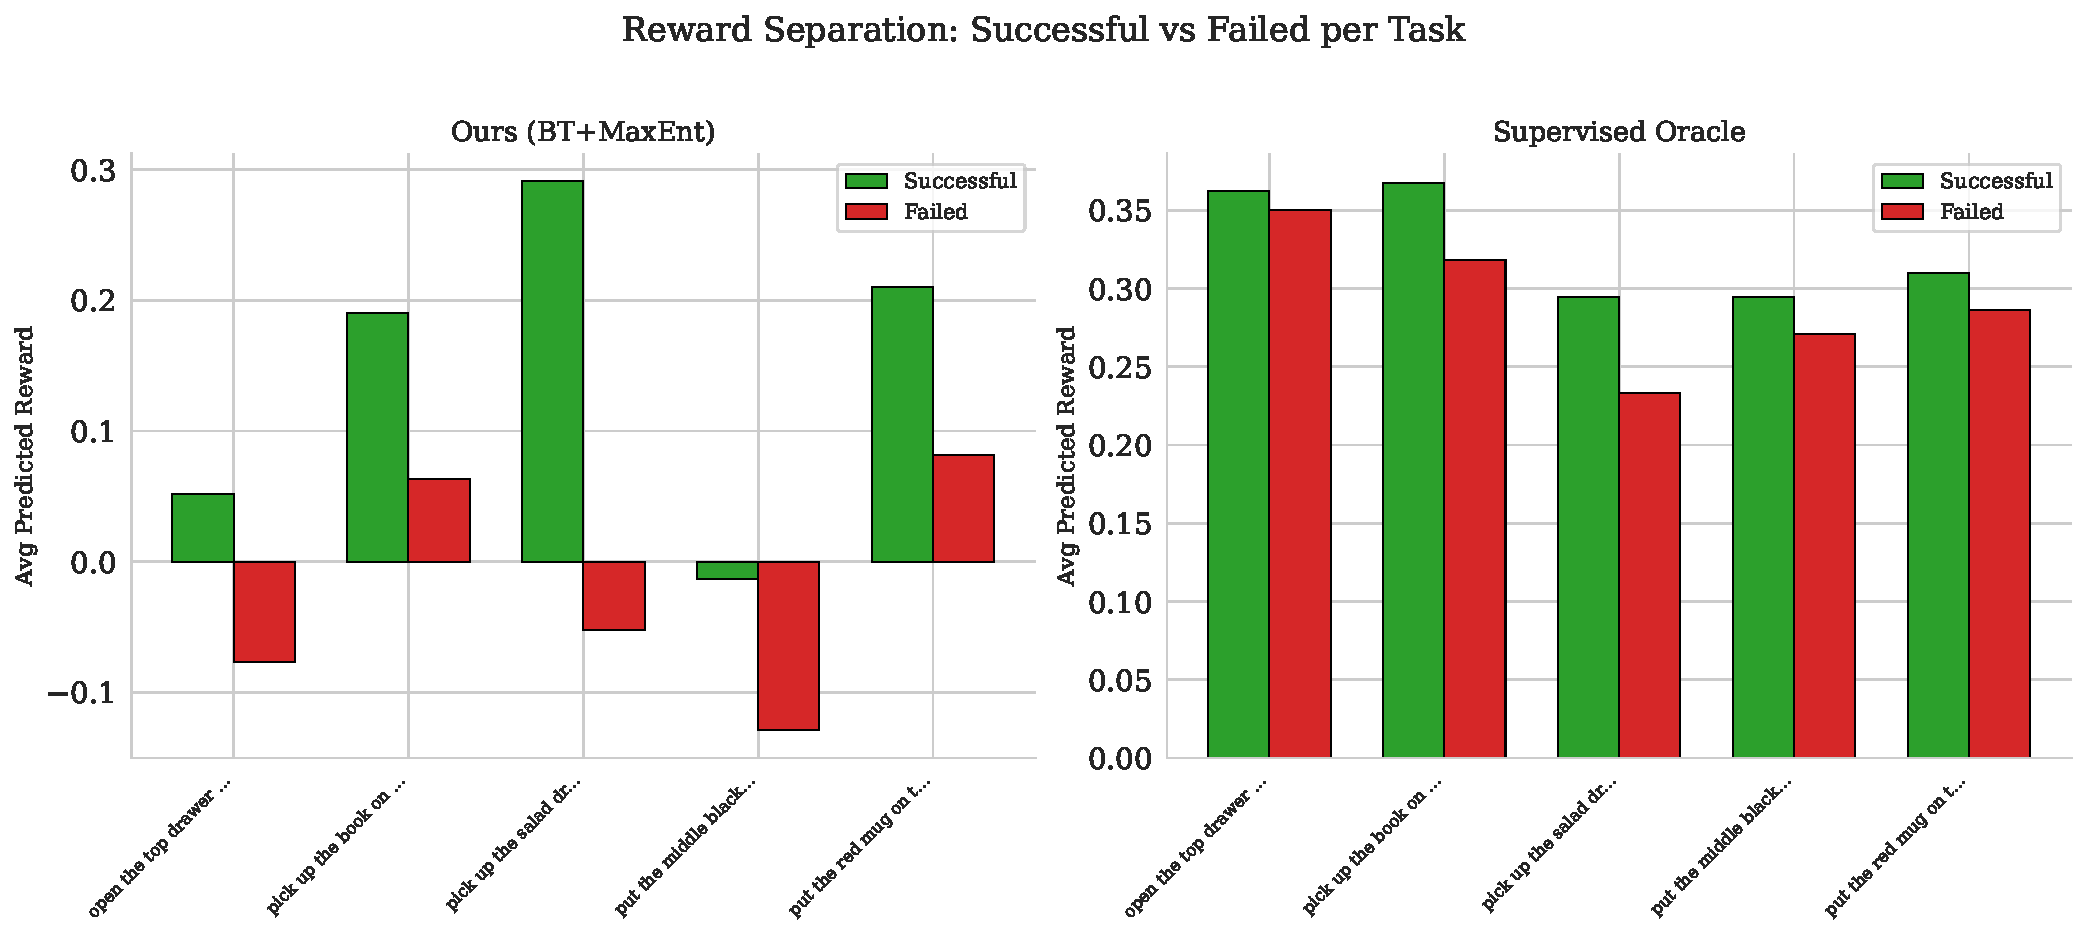
\includegraphics[width=0.95\textwidth]{figures/fig6_reward_separation_v3.pdf}
    \caption{本文方法与有监督基线在各任务上的奖励分离效果对比。绿色柱为成功轨迹的平均预测奖励，红色柱为失败轨迹。两种方法均可在所有任务上有效区分成败，但本文方法的分离幅度更大，为下游策略学习提供了更强的判别信号。}
    \label{fig:reward_separation}
\end{figure}

\subsection{分析}

\subsubsection{训练动态：避免梯度饱和}
\label{sec:training_dynamics}

将熵正则化直接施加于神经网络输出时，梯度饱和是一个常见风险。本文每条轨迹子采样8帧，相邻帧之间产生$T-1 = 7$个增量，因此均匀分布的理论最大熵为$\log 7 \approx 1.9459$。在早期实验中，基于Softplus的朴素公式使得$\mathcal{L}_{struct}$在训练伊始就饱和于$-\log 7 = -1.9459$，全程梯度为零。两处关键改进解决了这一问题：
\begin{enumerate}[leftmargin=*,noitemsep]
    \item \textbf{移除进度头的Sigmoid激活}，使势值无界化，为增量分布提供足够的方差空间。
    \item \textbf{引入温度参数$\alpha = 0.1$}。当$\alpha = 1.0$时，初始化阶段增量标准差仅约$0.2$，Softmax输出仍近似均匀，$\mathcal{L}_{struct}$停留在$-1.924$（占理论最大值的98.9\%），梯度信号极弱。将温度降至$\alpha = 0.1$后，增量差异被放大10倍，Softmax输出显著偏离均匀分布，$\mathcal{L}_{struct}$降至$-1.0 \sim -1.4$的工作区间，梯度信号恢复活跃。
\end{enumerate}

\cref{tab:dynamics}展示了两种模型设置下的训练动态。

\begin{table}[ht]
    \centering
    \caption{两种模型设置下$\mathcal{L}_{struct}$的训练动态。左半部分为Qwen3-VL-2B + LoRA（1250步），右半部分为SmolVLM-500M全参微调（1000步）。两者均表现出$\mathcal{L}_{struct}$远离饱和点、$\mathcal{L}_{BT}$正常收敛的一致趋势。}
    \label{tab:dynamics}
    \begin{tabular*}{\textwidth}{@{\extracolsep{\fill}}cccc|ccc@{}}
    \toprule
    \multicolumn{4}{c|}{\textbf{Qwen3-VL-2B + LoRA（1250步）}} & \multicolumn{3}{c}{\textbf{SmolVLM-500M 全参微调（1000步）}} \\
    \midrule
    \textbf{步数} & $\mathcal{L}_{struct}$ & $\mathcal{L}_{BT}$ & $\sigma^2(\Delta\Phi)$ & \textbf{步数} & $\mathcal{L}_{struct}$ & $\mathcal{L}_{BT}$ \\
    \midrule
    1 & $-1.003$ & 1.456 & 0.043 & 10 & $-1.158$ & 0.905 \\
    251 & $-1.167$ & 0.585 & --- & 100 & $-1.180$ & 0.655 \\
    501 & $-1.320$ & 0.594 & 0.029 & 500 & $-1.45 \sim -1.53$ & 0.121--0.178 \\
    651 & $-1.403$ & --- & --- & 1000 & $-1.55 \sim -1.56$ & 0.163--0.261 \\
    951 & $-1.140$ & 0.423 & 0.036 & & & \\
    \bottomrule
    \end{tabular*}
\end{table}

两种设置下趋势一致：$\mathcal{L}_{struct}$在$-1.0$到$-1.56$之间波动，远离饱和点$-\log 7 \approx -1.946$，梯度信号始终活跃。Qwen3设置下增量方差$\sigma^2(\Delta\Phi)$从$0.043$降至$0.029$--$0.036$，表明熵约束确实在推动增量趋于均匀。$\mathcal{L}_{BT}$在两种设置下均同步正常收敛，两个目标互不干扰。\cref{fig:training_dynamics}展示了完整的训练曲线。

\begin{figure}[htb]
    \centering
    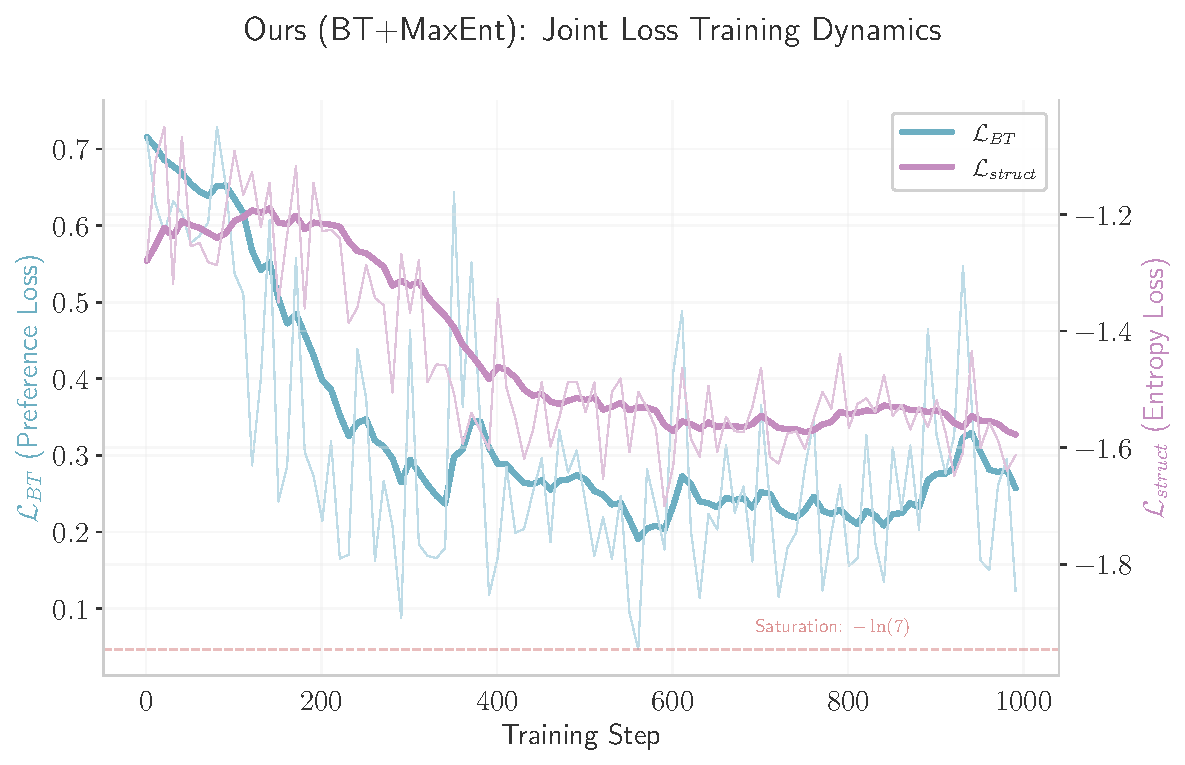
\includegraphics[width=0.65\textwidth]{figures/fig5_training_dynamics_v4_dual_axis.pdf}
    \caption{本文方法的联合训练动态（SmolVLM-500M全参微调）。蓝色曲线为偏好损失$\mathcal{L}_{BT}$（左轴），粉色曲线为结构损失$\mathcal{L}_{struct}$（右轴）。红色虚线标注了理论饱和点$-\ln 7 \approx -1.946$。$\mathcal{L}_{struct}$全程远离饱和点，梯度信号持续有效；$\mathcal{L}_{BT}$正常收敛，两个目标互不干扰。}
    \label{fig:training_dynamics}
\end{figure}

\begin{figure}[htb]
    \centering
    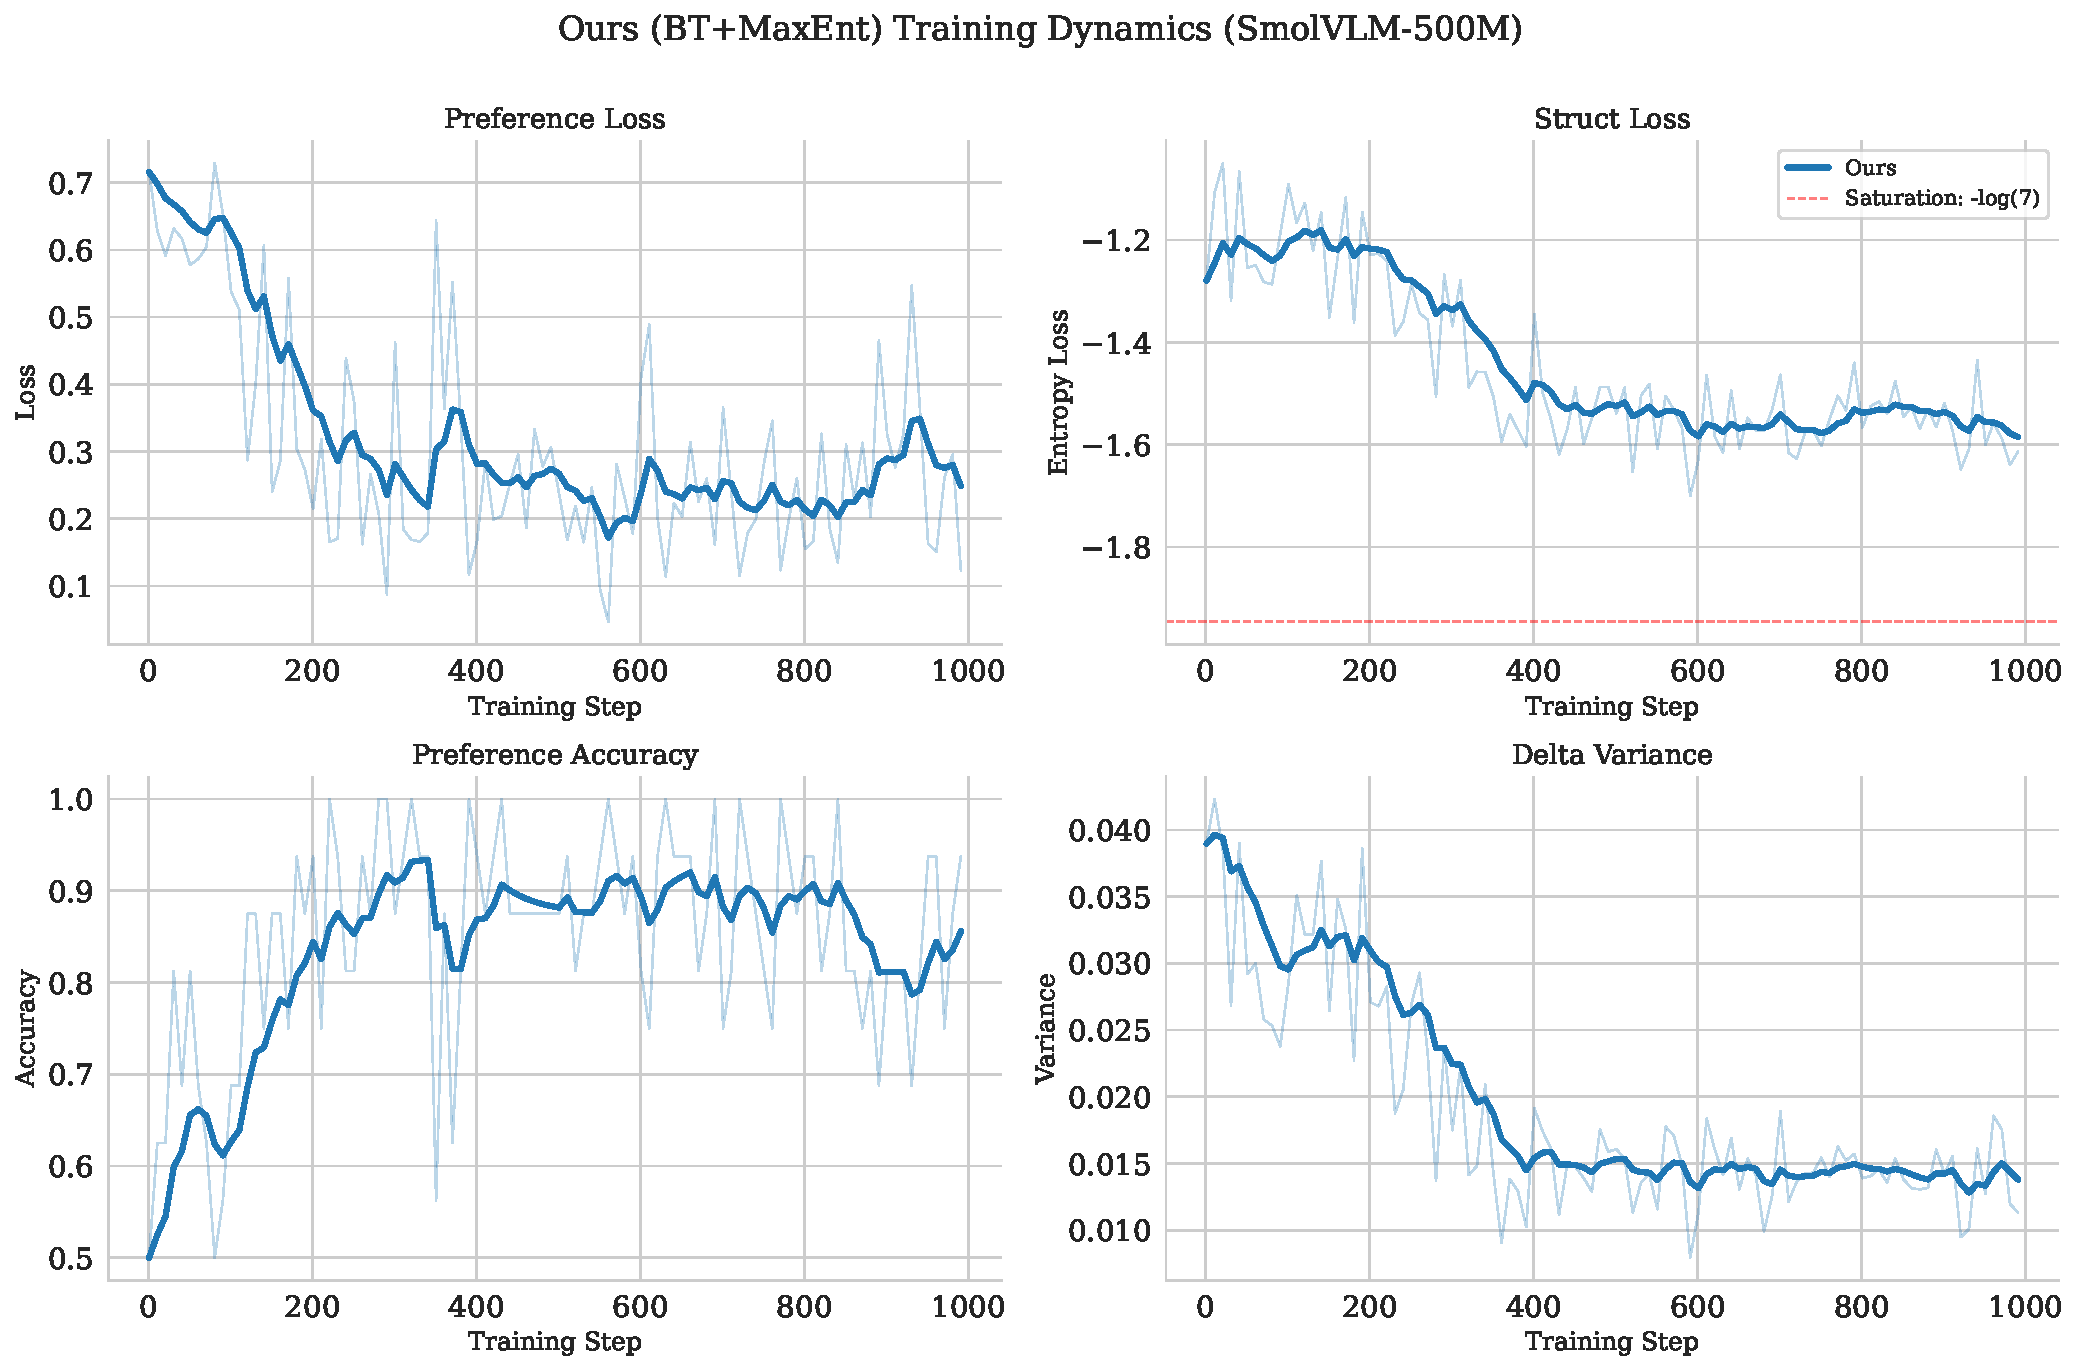
\includegraphics[width=0.95\textwidth]{figures/fig5_training_dynamics_v1.pdf}
    \caption{本文方法训练过程的四项关键指标：（左上）$\mathcal{L}_{BT}$持续收敛；（右上）$\mathcal{L}_{struct}$保持非饱和，梯度信号活跃；（左下）偏好预测准确率逐步提升至80\%以上；（右下）增量方差$\sigma^2(\Delta\Phi)$趋于稳定。}
    \label{fig:training_dynamics_detail}
\end{figure}

\subsubsection{方向歧义与$\mathcal{L}_{mono}$的作用}
\label{sec:direction}

移除Sigmoid激活后，势函数的单调方向不再有保证——它可能沿成功轨迹递减而非递增。这种方向歧义不影响轨迹级排序（BT损失对$\Phi$的全局符号不敏感），但会导致PBRS奖励信号方向反转。

$\mathcal{L}_{mono} = \text{mean}(\text{ReLU}(-\Delta\Phi_t))$通过惩罚负增量来解决这一问题。加入$\mathcal{L}_{mono}$后，本文方法在LIBERO-90上达到VOC $r = 0.968$，在LIBERO-10上达到$0.934$，均超过有监督基线的$0.860$。作为对照，不使用方向约束的纯BT基线VOC $r$仅为$0.147$，L2平滑为$0.616$——方向约束对帧级对齐至关重要。

训练日志证实了$\mathcal{L}_{mono}$的有效性：加入方向约束前，增量均值$\overline{\Delta\Phi}$在训练中始终为负（$-0.02 \sim -0.04$），模型学到了"均匀递减"的势函数；加入$\mathcal{L}_{mono}$后，增量均值在训练初期即翻转为正（$+0.01 \sim +0.06$），单调性惩罚项从初始的$0.076$稳步下降至$0.022$，表明负增量被有效抑制且未出现梯度消失。

\subsubsection{定性分析：轨迹关键帧与进度曲线}

\cref{fig:trajectory_frames}展示了代表性轨迹的关键帧及本文方法的进度预测。成功轨迹（绿色）的进度曲线平稳上升，反映出模型对任务完成度的准确感知；失败轨迹（红色）的进度停滞或偏低，符合预期。这表明$\mathcal{L}_{struct}$与$\mathcal{L}_{mono}$的结合不仅能在统计指标上取得优异表现，其学习到的势函数在物理语义层面也同样具有高度的合理性。

\begin{figure}[htb]
    \centering
    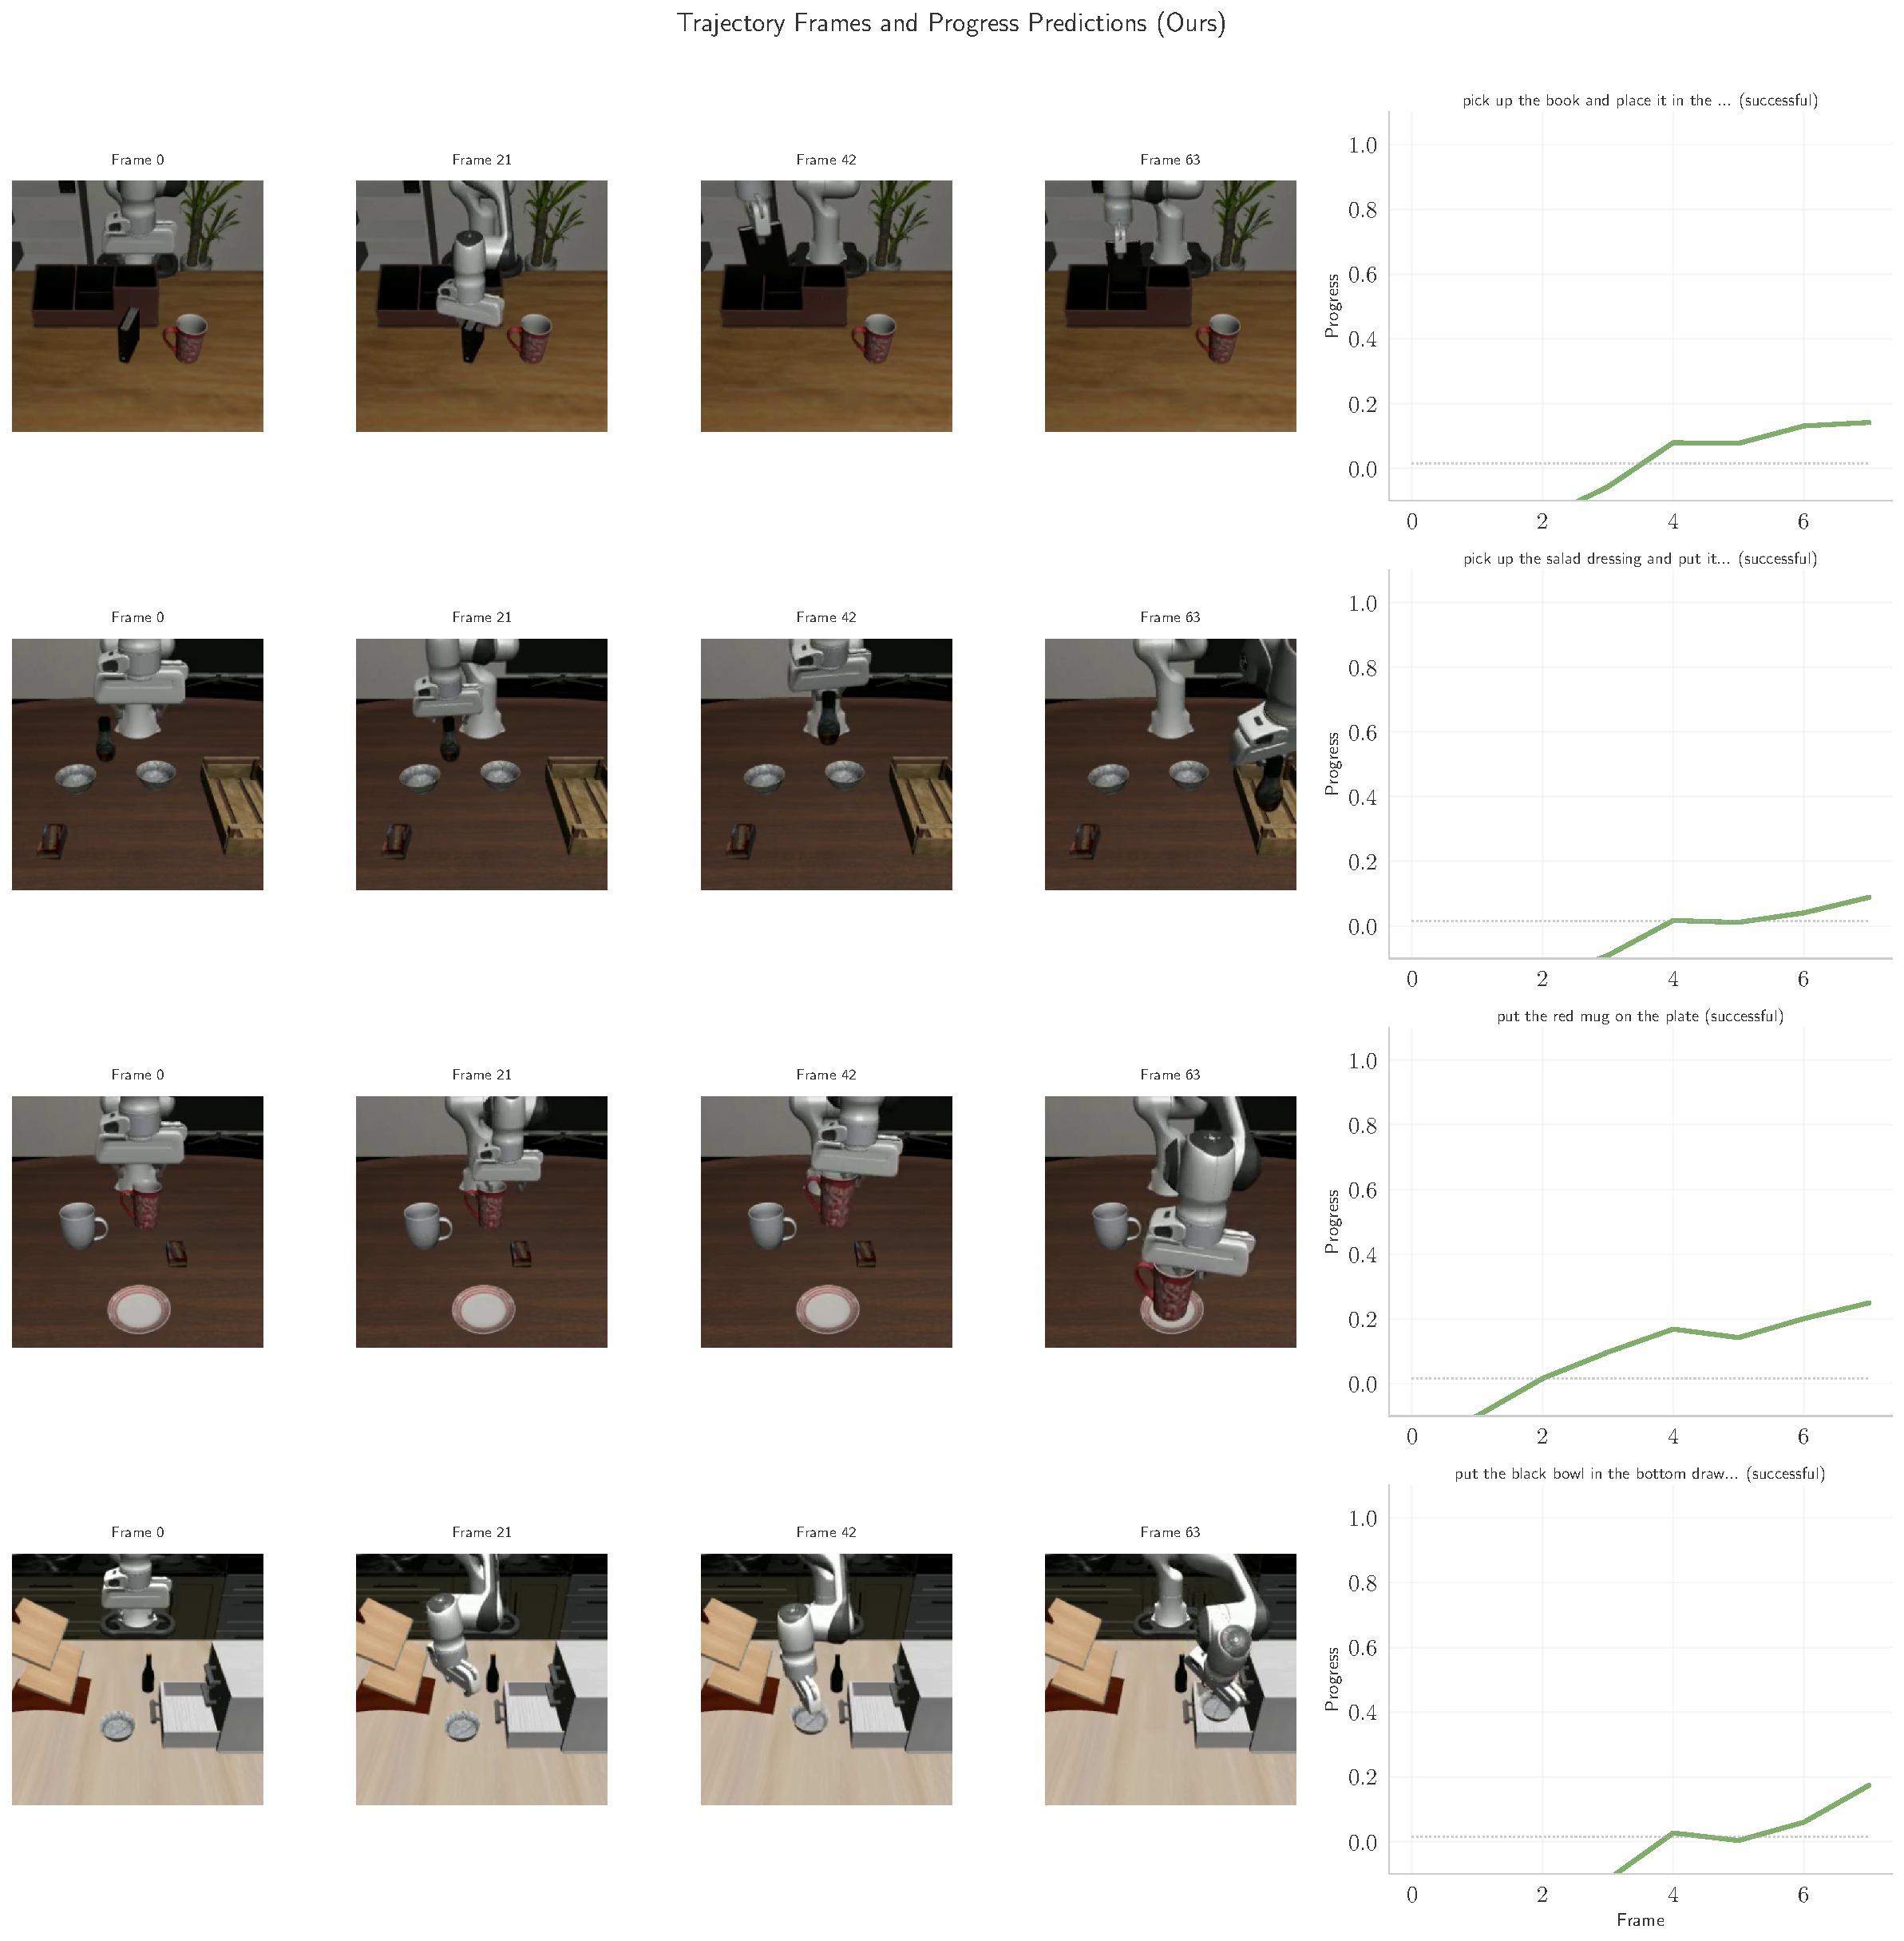
\includegraphics[width=0.95\textwidth]{figures/fig7_trajectory_frames_v1.pdf}
    \caption{代表性轨迹的关键帧与进度预测曲线。每行展示一条轨迹的四个等间距关键帧及本文方法的进度预测。成功轨迹（绿色）的进度平稳上升。}
    \label{fig:trajectory_frames}
\end{figure}


\subsection{下游策略学习实验}
\label{sec:policy_learning}

前述实验通过离线指标验证了本文奖励模型的帧级对齐质量和排序能力。本节进一步检验这些改进的增量结构能否在在线强化学习中转化为实际的策略性能提升。

\subsubsection{实验设置}

选取LIBERO-90基准中的Task 28（"close the top drawer of the cabinet"，关闭柜子顶部抽屉）作为测试任务，与ROBOMETER\cite{robometer2026}原文实验保持一致。策略算法采用Soft Actor-Critic（SAC）\cite{haarnoja2018}，使用DINOv2\cite{oquab2024dinov2} ViT-S/14提取384维视觉特征，拼接9维本体感受向量（关节角度 + 夹爪状态）构成393维的平坦观测空间，输入两层256维MLP构成的Actor和Critic网络。

奖励设计方面，比较两种方案：
\begin{itemize}[leftmargin=*,noitemsep]
    \item \textbf{BT+MaxEnt（本文方法）}：使用本文训练的奖励模型通过PBRS框架提供密集奖励信号。每一步的奖励为$r_t = \gamma\Phi(s_{t+1}) - \Phi(s_t)$，其中$\Phi$为奖励模型预测的进度势函数。
    \item \textbf{Sparse Reward（稀疏基线）}：仅使用环境原生的稀疏奖励——每步$-1$，任务成功时$0$。不加载VLM奖励模型。
\end{itemize}

主要超参数：折扣因子$\gamma = 0.99$，批大小256，学习率$3 \times 10^{-4}$，目标网络EMA系数$\tau = 0.005$，自动调节熵系数$\alpha$。每5000步在25条评估回合上测量成功率。

\subsubsection{结果与分析}

\cref{fig:rl_success_rate}展示了两种奖励方案下的策略学习曲线。

\begin{figure}[htb]
    \centering
    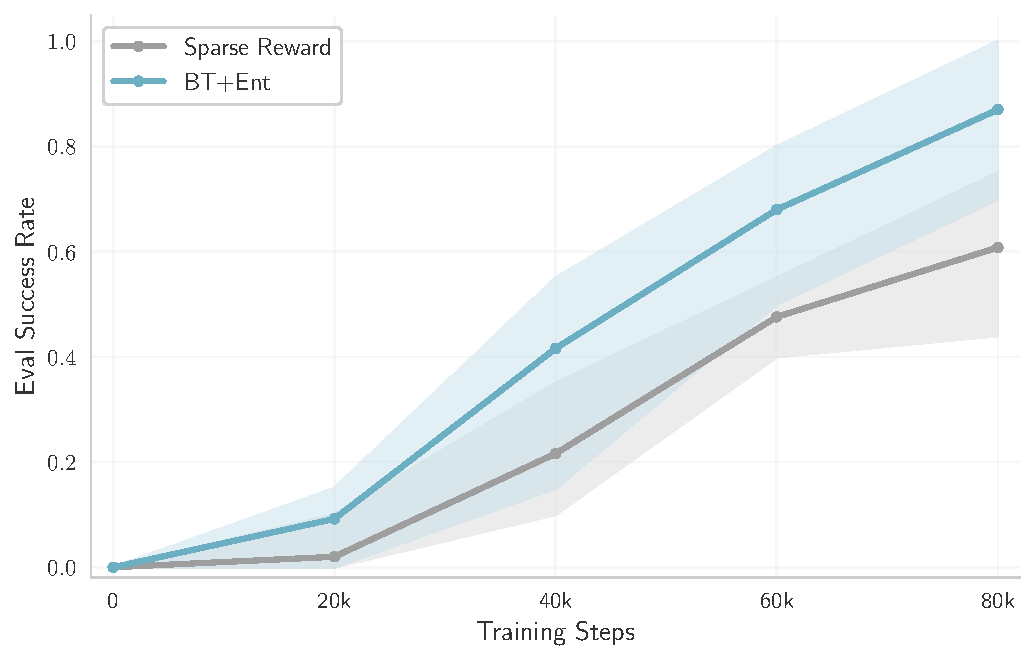
\includegraphics[width=0.85\textwidth]{figures/rl_success_rate.pdf}
    \caption{LIBERO-90 Task 28上的策略学习曲线：评估成功率随训练步数的变化。每20k steps做5次不同seed的eval。蓝色为本文BT+MaxEnt奖励模型（PBRS密集奖励），灰色为稀疏奖励基线。本文方法的密集奖励信号使策略更快地获得有意义的训练梯度。}
    \label{fig:rl_success_rate}
\end{figure}

本文提出的BT+MaxEnt奖励模型结合PBRS机制，能够在环境奖励稀疏、难以产生有效梯度的探索阶段，为下游策略优化输出持续且密集的学习信号。这一结果从端到端的角度验证了本文方法的实用价值：通过$\mathcal{L}_{struct}$和$\mathcal{L}_{mono}$改善的增量结构不仅在离线评估指标上优于基线（\cref{tab:main_results}），而且能够切实驱动下游策略学习。


\clearpage


\section{结论与展望}
\label{sec:conclusion}

本文揭示了基于偏好的奖励模型中一个此前被忽视的结构性问题——单调性陷阱：纯排序目标虽然能保证排序正确性，但无法约束PBRS部署所需的数值增量结构。为此，我们提出了最大熵增量约束（$\mathcal{L}_{struct}$），一种轻量的无监督正则化项，通过最大化时间增量分布的熵来规范势函数的增量结构，配合单调性铰链损失$\mathcal{L}_{mono}$确保增量方向正确。

LIBERO基准上的消融实验清晰地展示了各组件的作用：纯BT基线的轨迹级排序尚可（Kendall $\tau = 0.680$），但帧级对齐严重失调（VOC $r = 0.147$）；L2平滑有所改善（$0.616$）但仍不充分；本文方法将VOC $r$推至$0.968$，在帧级对齐上超越了使用帧级监督信号的有监督基线（$0.860$，提升$12.6\%$），轨迹级排序也全面领先（Kendall $\tau$：$0.696$ vs $0.504$，提升$38.1\%$）。这一结果验证了核心论点：仅从排序偏好就能恢复对RL友好的数值增量结构，无需获取成本高昂的帧级进度标注。

此外，下游策略学习实验（\cref{sec:policy_learning}）进一步表明，改善后的增量结构通过PBRS框架转化为有效的密集奖励信号，在LIBERO-90 Task 28上显著优于稀疏奖励基线。

\textbf{未来工作。}将方法推广到更多LIBERO任务和真实机器人平台，以及探索更大规模VLM模型的奖励建模能力，是重要的后续研究方向。



\clearpage
\begin{thebibliography}{99}

    \bibitem{abdelkareem2022advances}
    Abdelkareem Y, Shehata S, Karray F.
    Advances in Preference-based Reinforcement Learning: A Review[C].
    2022 IEEE International Conference on Systems, Man, and Cybernetics (SMC), 2022: 2527--2532.
    
    \bibitem{muller2025improving}
    Müller H, Kudenko D.
    Improving the Effectiveness of Potential-Based Reward Shaping in Reinforcement Learning[C].
    Proceedings of the 24th International Conference on Autonomous Agents and Multiagent Systems (AAMAS), 2025: 2684--2686.
    
    \bibitem{trajectory2024comparativelanguage}
    Yang Z, Jun M, Tien J, Russell S J, Dragan A, Biyik E.
    Trajectory Improvement and Reward Learning from Comparative Language Feedback[C].
    Proceedings of the 8th Annual Conference on Robot Learning (CoRL), 2024.
    
    \bibitem{christiano2017deep}
    Christiano P F, Leike J, Brown T B, Martic M, Legg S, Amodei D.
    Deep Reinforcement Learning from Human Preferences[C].
    Advances in Neural Information Processing Systems, 2017, 30.
    
    \bibitem{brown2019extrapolating}
    Brown D S, Goo W, Nagarajan P, Niekum S.
    Extrapolating Beyond Suboptimal Demonstrations via Inverse Reinforcement Learning from Observations[C].
    Proceedings of the 36th International Conference on Machine Learning (ICML), 2019: 783--792.
    
    \bibitem{lee2021bpref}
    Lee K, Smith L M, Dragan A, Abbeel P.
    B-Pref: Benchmarking Preference-Based Reinforcement Learning[C].
    Advances in Neural Information Processing Systems, 2021, 34.
    
    \bibitem{park2022surf}
    Park J, Seo Y, Shin J.
    SURF: Semi-Supervised Reward Learning with Data Augmentation for Feedback-Efficient Preference-Based Reinforcement Learning[C].
    International Conference on Learning Representations (ICLR), 2022.
    
    \bibitem{robometer2026}
    Liang A, Korkmaz Y, Zhang J, Hwang M, Anwar A, Kaushik S, Shah A, Huang A S, Zettlemoyer L, Fox D, Xiang Y, Li A, Bobu A, Gupta A, Tu S, Biyik E, Zhang J.
    Robometer: Scaling General-Purpose Robotic Reward Models via Trajectory Comparisons[C].
    Robotics: Science and Systems (RSS), 2026.
    
    \bibitem{krack2026rewarding}
    Krack P, Jülg T, Burgard W, Walter F.
    Rewarding DINO: Predicting Dense Rewards with Vision Foundation Models[OL].
    arXiv preprint arXiv:2603.16978, 2026.
    
    \bibitem{ng1999policy}
    Ng A Y, Harada D, Russell S.
    Policy Invariance Under Reward Transformations: Theory and Application to Reward Shaping[C].
    Proceedings of the 16th International Conference on Machine Learning (ICML), 1999: 278--287.
    
    \bibitem{fu2018airl}
    Fu J, Luo K, Levine S.
    Learning Robust Rewards with Adversarial Inverse Reinforcement Learning[C].
    International Conference on Learning Representations (ICLR), 2018.
    
    \bibitem{ibarz2018reward}
    Ibarz B, Leike J, Pohlen T, Irving G, Legg S, Amodei D.
    Reward Learning from Human Preferences and Demonstrations in Atari[C].
    Advances in Neural Information Processing Systems, 2018, 31.
    
    \bibitem{lee2021pebble}
    Lee K, Smith L M, Abbeel P.
    PEBBLE: Feedback-Efficient Interactive Reinforcement Learning via Relabeling Experience and Unsupervised Pre-training[C].
    Proceedings of the 38th International Conference on Machine Learning (ICML), 2021.
    
    \bibitem{kumar2020d4rl}
    Fu J, Kumar A, Nachum O, Tucker G, Levine S.
    D4RL: Datasets for Deep Data-Driven Reinforcement Learning[OL].
    arXiv preprint arXiv:2004.07219, 2020.
    
    \bibitem{yu2020metaworld}
    Yu T, Quillen D, He Z, Julian R, Narayan A, Shively H, Bellathur A, Hausman K, Finn C, Levine S.
    Meta-World: A Benchmark and Evaluation for Multi-Task and Meta Reinforcement Learning[C].
    Conference on Robot Learning (CoRL), 2019.
    
    \bibitem{radford2021clip}
    Radford A, Kim J W, Hallacy C, Ramesh A, Goh G, Agarwal S, Sastry G, Askell A, Mishkin P, Clark J, Krueger G, Sutskever I.
    Learning Transferable Visual Models From Natural Language Supervision[C].
    Proceedings of the 38th International Conference on Machine Learning (ICML), 2021.
    
    \bibitem{nair2022r3m}
    Nair S, Rajeswaran A, Kumar V, Finn C, Gupta A.
    R3M: A Universal Visual Representation for Robot Manipulation[C].
    Conference on Robot Learning (CoRL), 2022.
    
    \bibitem{ma2023vip}
    Ma Y J, Sodhani S, Jayaraman D, Bastani O, Kumar V, Zhang A.
    VIP: Towards Universal Visual Reward and Representation via Value-Implicit Pre-Training[C].
    International Conference on Learning Representations (ICLR), 2023.
    
    \bibitem{ma2023liv}
    Ma Y J, Kumar V, Zhang A, Bastani O, Jayaraman D.
    LIV: Language-Image Representations and Rewards for Robotic Control[C].
    Proceedings of the 40th International Conference on Machine Learning (ICML). PMLR, 2023, 202: 23301--23320.
    
    \bibitem{sontakke2023roboclip}
    Sontakke S A, Zhang J, Arnold S M R, Pertsch K, Biyik E, Sadigh D, Finn C, Itti L.
    RoboCLIP: One Demonstration is Enough to Learn Robot Policies[C].
    Advances in Neural Information Processing Systems, 2023, 36.

    \bibitem{ma2024eureka}
    Ma Y J, Liang W, Wang G, Huang D A, Bastani O, Jayaraman D, Zhu Y, Fan L, Anandkumar A.
    Eureka: Human-Level Reward Design via Coding Large Language Models[C].
    International Conference on Learning Representations (ICLR), 2024.
    
    \bibitem{ouyang2022training}
    Ouyang L, Wu J, Jiang X, Almeida D, Wainwright C L, Mishkin P, Zhang C, Agarwal S, Slama K, Ray A, Schulman J, Hilton J, Kelton F, Miller L, Simens M, Askell A, Welinder P, Christiano P, Leike J, Lowe R.
    Training Language Models to Follow Instructions with Human Feedback[C].
    Advances in Neural Information Processing Systems, 2022, 35: 27730--27744.
    
    \bibitem{oquab2024dinov2}
    Oquab M, Darcet T, Moutakanni T, Vo H, Szafraniec M, Khalidov V, Fernandez P, Haziza D, Massa F, El-Nouby A, Howes R, Huang P Y, Xu H, Sharma V, Li S W, Galuba W, Rabbat M, Assran M, Ballas N, Synnaeve G, Misra I, Jegou H, Mairal J, Labatut P, Joulin A, Bojanowski P.
    DINOv2: Learning Robust Visual Features without Supervision[J].
    Transactions on Machine Learning Research, 2024.
    
    \bibitem{liang2022rune}
    Liang X, Shu K, Lee K, Abbeel P.
    Reward Uncertainty for Exploration in Preference-based Reinforcement Learning[C].
    International Conference on Learning Representations (ICLR), 2022.
    
    \bibitem{ho2016gail}
    Ho J, Ermon S.
    Generative adversarial imitation learning[C].
    Advances in Neural Information Processing Systems, 2016, 29.
    
    \bibitem{finn2016guided}
    Finn C, Levine S, Abbeel P.
    Guided cost learning: Deep inverse optimal control via policy optimization[C].
    Proceedings of the 33rd International Conference on Machine Learning, 2016: 49--58.
    
    \bibitem{ziebart2008maximum}
    Ziebart B D, Maas A L, Bagnell J A, Dey A K.
    Maximum entropy inverse reinforcement learning[C].
    Proceedings of the AAAI Conference on Artificial Intelligence, 2008, 8: 1433--1438.
    
    \bibitem{reddy2020sqil}
    Reddy S, Dragan A D, Levine S.
    SQIL: Imitation learning via reinforcement learning with sparse rewards[C].
    International Conference on Learning Representations, 2020.
    
    \bibitem{rajeswaran2018dapg}
    Rajeswaran A, Kumar V, Gupta A, Vezzani G, Schulman J, Todorov E, Levine S.
    Learning complex dexterous manipulation with deep reinforcement learning and demonstrations[C].
    Robotics: Science and Systems, 2018.
    
    \bibitem{shridhar2022cliport}
    Shridhar M, Manuelli L, Fox D.
    CLIPort: What and where pathways for robotic manipulation[C].
    Conference on Robot Learning, 2022.
    
    \bibitem{mandlekar2021robomimic}
    Mandlekar A, Xu D, Wong J, Nasiriany S, Wang C, Kulkarni R, Fei-Fei L, Savarese S, Zhu Y, Martin-Martin R.
    What matters in learning from offline human demonstrations for robot manipulation[C].
    Conference on Robot Learning, 2021.
    
    \bibitem{mandlekar2023mimicgen}
    Mandlekar A, Nasiriany S, Wen B, Akinola I, Narang Y S, Fan L, Zhu Y, Fox D.
    MimicGen: A data generation system for scalable robot learning using human demonstrations[C].
    Conference on Robot Learning, 2023.
    
    \bibitem{zhu2020robosuite}
    Zhu Y, Wong J, Mandlekar A, Martin-Martin R, Joshi A, Lin K, Maddukuri A, Nasiriany S, Zhu Y.
    robosuite: A Modular Simulation Framework and Benchmark for Robot Learning[OL].
    arXiv preprint arXiv:2009.12293, 2020.
    
    \bibitem{liu2023libero}
    Liu B, Zhu Y, Gao C, Feng Y, Liu Q, Zhu Y, Stone P.
    LIBERO: Benchmarking Knowledge Transfer for Lifelong Robot Learning[C].
    Advances in Neural Information Processing Systems, 2023, 36.

    \bibitem{shannon1948}
Shannon C E.
A mathematical theory of communication[J].
The Bell System Technical Journal, 1948, 27(3): 379--423; 27(4): 623--656.

\bibitem{jaynes1957}
Jaynes E T.
Information theory and statistical mechanics[J].
Physical Review, 1957, 106(4): 620--630.


\bibitem{zhao2025}
Zhao D, Wang R, Suh D, Kim T, Yuan Z, Min B-C, Chen G.
PrefMMT: Modeling Human Preferences in Preference-based Reinforcement Learning with Multimodal Transformers[C].
Proceedings of the IEEE/RSJ International Conference on Intelligent Robots and Systems (IROS), 2025: 18692--18699.

\bibitem{bradley1952}
Bradley R A, Terry M E.
Rank analysis of incomplete block designs: I. The method of paired comparisons[J].
Biometrika, 1952, 39(3/4): 324--345.


\bibitem{schulman2017}
Schulman J, Wolski F, Dhariwal P, Radford A, Klimov O.
Proximal Policy Optimization Algorithms[OL].
arXiv preprint arXiv:1707.06347, 2017.

\bibitem{haarnoja2018}
Haarnoja T, Zhou A, Abbeel P, Levine S.
Soft actor-critic: Off-policy maximum entropy deep reinforcement learning with a stochastic actor[C].
Proceedings of the 35th International Conference on Machine Learning. PMLR, 2018, 80: 1861--1870.

\bibitem{marafioti2025smolvlm}
Marafioti A, Zohar O, Farre M, et al.
SmolVLM: Redefining Small and Efficient Multimodal Models[OL].
arXiv preprint arXiv:2504.05299, 2025.

\bibitem{ma2024generative}
Ma Y J, Hejna J, Fu C, Shah D, Liang J, Xu Z, Kirmani S, Xu P, Driess D, Xiao T, Bastani O, Jayaraman D, Yu W, Zhang T, Sadigh D, Xia F.
Vision Language Models are In-Context Value Learners[C].
International Conference on Learning Representations (ICLR), 2025.

\bibitem{sutton2018}
Sutton R S, Barto A G.
Reinforcement Learning: An Introduction[M].
2nd ed. Cambridge, MA: MIT Press, 2018.


\end{thebibliography}



\clearpage
\section*{致谢}

感谢吴祖煊老师在研究方向和论文写作上的悉心指导。感谢ROBOMETER\cite{robometer2026}开源代码库为本工作提供的实验基础设施。本研究使用的计算资源由AutoDL云平台提供。


\end{document}
